\chapter{Aplicaciones entre Espacios Topológicos}

\begin{definicion}
    Dados $(X, \cc{T})$, $(Y, \cc{T}')$ dos e.t., diremos que $f : (X, \cc{T}) \to (Y, \cc{T}')$ (que notaremos como $f:X \to Y$ cuando estén claros los e.t.) es \textbf{continua} en un punto $x_0\in X$ si $\forall N'\in \cc{N}_{f(x_0)}'$ existe un entorno $ N \in \cc{N}_{x_0}$ con $f(N)\subset N'$. 

    \begin{center}
        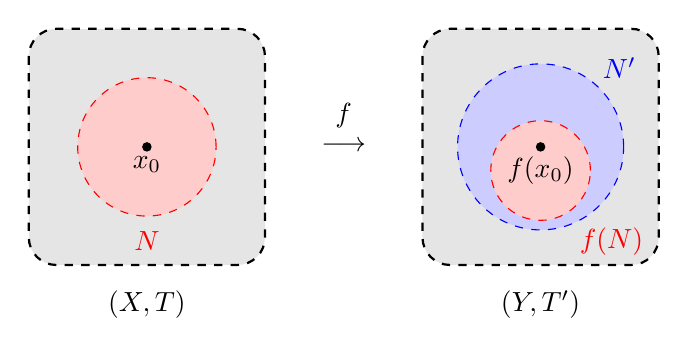
\begin{tikzpicture}
            \def\incolor{gray!20}

            \filldraw[rounded corners=10pt, dashed, thick, fill=\incolor] (0,0) rectangle (3,-3);

            \node at (1.5, -3.5) {$(X, \cc{T})$};
            \node at (4, -1.1) {$f$};
            \node at (4, -1.5) {$\longrightarrow$};

            \filldraw[rounded corners=10pt, dashed, thick, fill=\incolor] (5,0) rectangle (8,-3);

            \node at (6.5, -3.5) {$(Y, \cc{T}')$};

            \filldraw[dashed, draw=red, fill=red!20] (1.5, -1.5) circle (25pt);

            \node at (1.5, -2.7) {\textcolor{red}{$N$}};

            \filldraw[dashed, draw=blue, fill=blue!20] (6.5, -1.5) circle (30pt);

            \filldraw[dashed, draw=red, fill=red!20] (6.5, -1.8) circle (18pt);

            \node at (7.4, -2.7) {\textcolor{red}{$f(N)$}};

            \node at (7.5, -0.5) {\textcolor{blue}{$N'$}};

            \filldraw (1.5, -1.5) circle (1.5pt)  node[below] {$x_0$};

            \filldraw (6.5, -1.5) circle (1.5pt)  node[below] {$f(x_0)$};

            
        \end{tikzpicture}
    \end{center}

    Equivalentemente, $\forall N'\in \cc{N}_{f(x)}'$ se tiene que  $f^{-1}(N')\in \cc{N}_{x_0}$. Es decir, la imagen inversa por f de todo entorno de $f(x)$ en el espacio topológico $\cc{T}'$ es entorno de $x$ en el espacio topológico $\cc{T}$.
    \endsquare
\end{definicion}

\begin{observacion}
    La definición se puede reformular usando abiertos, abiertos básicos o entornos básicos. La demostración queda planteada como ejercicio para el lector. %TODO
    \endsquare
\end{observacion}

\begin{definicion}
    Dados $(X, \cc{T})$, $(Y, \cc{T}')$ dos e.t., $\emptyset \neq A\subset X$. Diremos que $f:X\to Y$ es \textbf{continua en $A$} si es continua en $x$\ \ $\forall x \in A$. Diremos que $f$ es \textbf{continua} si es continua en $X$.
    \endsquare
\end{definicion}

\begin{prop}
    Dados $(X, \cc{T})$, $(Y, \cc{T}')$ dos e.t., $f: X \to Y$. Entonces son equivalentes:
    \begin{enumerate}
        \item[(i)] $f$ es continua.
        \item[(ii)] $f^{-1}(U')\in \cc{T}$\ \ $\forall U' \in \cc{T}$ ($f$ trae abiertos en abiertos).
        \item[(iii)] $f^{-1}(B')\in \cc{T}$\ \ $\forall B'\in \cc{B}'$, donde $\cc{B}'$ es base de $\cc{T}'$.
        \item[(iv)] $f^{-1}(C')\in \cc{C}_{\cc{T}}$\ \ $\forall C' \in \cc{C}_{\cc{T}'}$ ($f$ trae cerrados en cerrados).
        \item[(v)] $f(\overline{A})\subset \overline{f(A)}$\ \ $\forall A \subset X$.
    \end{enumerate}

    \begin{proof}\
        \begin{enumerate}
            \item[(i)$\Rightarrow$(ii) )] Supongamos que $f$ es continua. Tomamos $U' \in \cc{T}'$ y tendremos que verificar que $f^{-1}(U')\in \cc{T}$. Sea $x \in f^{-1}(U')$, entonces tendré que ver que $f^{-1}(U')\in \cc{N}_x$. Sabemos que $f(x)\in U' \subset \cc{N}_{f(x)}$. Como $f$ es continua, entonces $\exists U\in \cc{T} $, $x\in U$, $f(U)\subset U' \Rightarrow x \in U \subset f^{-1}(U')$. Como $U\in \cc{T}$, tenemos que $f^{-1}(U')\in \cc{N}_x$. Como esto sucede para un $x$ arbitrario tendremos que se verifica.
            \item[(ii)$\Rightarrow$(iii) )] Esta implicación es trivial ya que todo abierto básico es en particular abierto en la topología.
            \item[(iii)$\Rightarrow$(iv) )] Sea $C' \in \cc{C}_{\cc{T}'}$, $C'\subset Y$. Tendré que ver que $f^{-1}(C')\in \cc{C}_{\cc{T}}$, lo cual es equivalente a ver que $X \setminus f^{-1}(C')\in \cc{T}$. Sabemos que $X\setminus f^{-1}(C') = f^{-1}(Y\setminus C')$ y $Y\setminus C'\in \cc{T}$. Como $\cc{B}'$ es base de $\cc{T}'$, tenemos que $Y\setminus C'=\bigcup\limits_{i\in I} B_i'$ con $B_i'\in \cc{B}'$\ \ $\forall i \in I$. Entonces tenemos que $f^{-1}(Y\setminus C') = f^{-1}\left(\bigcup\limits_{i\in I}B_i'\right) = \bigcup\limits_{i\in I}f^{-1}(B_i')\in \cc{T}$ por ser unión de abiertos.
            \item[(iv)$\Rightarrow$(v) )] Sea $\emptyset \neq A \subset X$, como $\overline{f(A)}\in \cc{C}_{\cc{T}'}$, por (iv) tenemos que $f^{-1}(\overline{f(A)})\in \cc{C}_{\cc{T}}$. Además, $A \subset f^{-1}(f(A))\subset f^{-1}(\overline{f(A)})\in \cc{C}_{\cc{T}}$. Entonces $\overline{A}\subset f^{-1}(\overline{f(A)})$. Al aplicar $f$ tenemos que $f(\overline{A})\subset f(f^{-1}(\overline{f(A)}))=\overline{f(A)}$.
            \item[(v)$\Rightarrow$(iv) )] Sea $C' \in \cc{C}_{\cc{T}'}$ y tendremos que ver que $f^{-1}(C')\in \cc{C}_{\cc{T}}$. Para ello veré que coincide con su adherencia, es decir, que $\overline{f^{-1}(C')} = f^{-1}(C')$. Como la inclusión $\overline{f^{-1}(C')} \supset f^{-1}(C')$ es clara tendré que ver solo la otra incusión. Sea $A=f^{-1}(C')$, por (v) tenemos que $f(\overline{f^{-1}(C')})\subset \overline{f(f^{-1}(C'))} \subset \overline{C'}=C'$. Aplicando $f^{-1}$ tenemos que $f^{-1}(f(\overline{f^{-1}(C')}))\subset f^{-1}(C')$ y como $f^{-1}(f(\overline{f^{-1}(C')})) = \overline{f^{-1}(C')}$ tenemos lo buscado.
            \item[(iv)$\Rightarrow$(i) )] Sea $x\in X$ arbitrario. Tendré que ver que $f$ es continua en $x$. Sea $U'\in \cc{T}'$ con $f(x)\in U'$. Tendré que ver que existe un $U\in \cc{T}$ con $x\in U$ y $f(U)\subset U'$. Tomo $Y\setminus(U')\in \cc{C}_{\cc{T}'}$ y por (iv) tenemos que $f^{-1}(Y\setminus U')\in \cc{C}_{\cc{T}}$ y $f^{-1}(Y\setminus U') = X \setminus f^{-1}(U')$ por lo que $x\in f^{-1}(U')\in \cc{T}$. Como $f(f^{-1}(U'))\subset U'$ puedo denotar $U = f^{-1}(U')$ y tenemos de nuevo lo buscado. 
        \end{enumerate}
    \end{proof}
\end{prop}

\begin{observacion}
    Si $f: (X, \cc{T}) \to (\bb{R}, \cc{T}_u)$ es una aplicación continua, entonces 
    \begin{gather*}
        f^{-1}((a,b)), f^{-1}((-\infty, b)), f^{-1}((a, +\infty))\in \cc{T}
    \end{gather*}
    y además 
    \begin{gather*}
        f^{-1}([a,b]), f^{-1}((-\infty, b]), f^{-1}([a, +\infty))\in \cc{C}_{\cc{T}}
    \end{gather*}
    La utilidad de esta observación es poder ver si un conjunto es abierto viendo si existe una aplicación continua que lleve un abierto de la topología en dicho conjunto. Análogamente se puede usar para cerrados.
    \endsquare
\end{observacion}

\begin{ejemplo}\
    \begin{itemize}
        \item $f:(X, d) \to (Y, d')$ continua entre espacios métricos 
        \begin{align*}
            \sii &\forall \veps >0\ \ \exists \delta >0 \text{ tal que si } d(x, x_0)<\delta \text{ entonces } d'(f(x), f(x_0))<\veps \sii\\
            \sii &\forall \veps >0 \ \ \exists \delta >0 \text{ tal que } f(B(x_0, \delta))\subset B'(f(x_0), \veps).
        \end{align*}
    \end{itemize}
    \endsquare
\end{ejemplo}

\begin{observacion}\
    \begin{itemize}
        \item Cuanto más abiertos hay en $\cc{T}$ y menos en $\cc{T}'$ se puede decir que es ``más fácil'' que $f$ sea continua. Por ejemplo, las aplicaciones  
        \begin{align*}
            f:&(X, \cc{T})\to (Y, \cc{T}_t)\\
            f:&(X, \cc{T}_{disc})\to (Y, \cc{T}')
        \end{align*}
        son continuas siempre.

        \item Si $f:(X, \cc{T})\to (Y, \cc{T}')$ es constante, es decir, $f(x)=y_0\in Y$\ \ $\forall x \in X$, entonces para todo $U'\in \cc{T}$ se tiene 
        \begin{gather*}
            f^{-1}(U')=\left\{
            \begin{array}{ccc}
                X & \text{ si }& y_0\in U'\\
                \emptyset & \text{ si } & y_0\notin U
            \end{array}
            \right.
        \end{gather*}
        y por tanto $f$ es continua ya que $X, \emptyset \in \cc{T}$.

        \item $Id_X : (X, \cc{T}) \to (X, \cc{T}')$ es continua $\sii \cc{T}' \leq \cc{T}$. Por ejemplo, 
        \begin{align*}
            Id_{\bb{R}}:(\bb{R}, \cc{T}_u)\to (\bb{R}, \cc{T}_S)
        \end{align*}
        no es continua pero
        \begin{align*}
            Id_{\bb{R}}:(\bb{R}, \cc{T}_S) \to (\bb{R}, \cc{T}_u)
        \end{align*} 
        sí lo es.
        \item Si $f:(X, \cc{T})\to (Y, \cc{T}')$ y $g:(Y, \cc{T}')\to (Z, \cc{T}'')$ son aplicaciones continuas, entonces $g\circ f : (X, \cc{T})\to (Z, \cc{T}'')$ es continua.
        \begin{proof}
            Sea $U''\in \cc{T}''$, $(g\circ f)^{-1}(U'') = f^{-1}(g^{-1}(U''))\in \cc{T}$.
        \end{proof}
        \item $f:(X, \cc{T})\to (Y,\cc{T}')$ continua y $\emptyset\neq A  \subset X$, entonces
        \begin{align*}
            f|_{A}:(A, \cc{T}_A) &\to (Y, \cc{T}') \text{ es continua}\\
            x & \mapsto f(x)
        \end{align*}
        es decir, la restricción en el dominio de una función continua sigue siendo continua.
        \begin{proof}
            Sea $U'\in \cc{T}'$, entonces 
            \begin{align*}
                (f|_{A})^{-1}(U') = \{x \in A : f(x)\in U\} = f^{-1}(U') \cap A\in \cc{T}_A
            \end{align*}
            ya que $f^{-1}(U')\in \cc{T}$.
        \end{proof}
        \item Si $f:(X, \cc{T})\to (Y, \cc{T}')$ continua, $\emptyset \neq A' \subset Y$ con $f(X)\subset A'$, entonces 
        \begin{align*}
            f^{A'}:(X, \cc{T}) &\to (A', \cc{T}_{A'}') \text{ es continua}\\
            x &\mapsto f(x)
        \end{align*}
        es decir, la restricción en el codominio de una función continua sigue siendo continua.
        \begin{proof}
            Sea $O'\in \cc{T}_{A'}'$, entonces $\exists U'\in \cc{T}'$ tal que  $O'=U'\cap A \Rightarrow (f^{A'})^{-1}(O') = (f^{A'})^{-1}(U'\cap A') = f^{-1}(U')\in \cc{T}$ ya que $f$ es continua y $U'$ es abierto en $\cc{T}'$.

        \end{proof}
    \end{itemize}
\end{observacion}

\begin{lema} (Lema de pegado) Sean $(X, \cc{T})$, $(Y, \cc{T}')$ dos e.t. y sea $\{A_i\}_{i\in I}\subset X$ una familia de subconjuntos no vacía de $X$ y $\{f_i:A_i \to Y\}_{i\in I}$ una familia de aplicaciones tales que 
    \begin{enumerate}
        \item[(i)] $\bigcup\limits_{i\in I} A_i =X$.
        \item[(ii)] $f_i=f_j$ en $A_i\cap A_j$\ \ $\forall i,j\in I$ con $A_i\cap A_j \neq \emptyset$. 
        \item[(iii)] $f_i:(A_i, \cc{T}_{A_i})\to (Y, \cc{T}')$ es continua $\forall i \in I$. 
        \item[(iv)] O bien $A_i\in \cc{T}$\ \ $\forall i \in I$ o bien $A_i \in \cc{C}_{\cc{T}}$\ \ $\forall i \in I$ con $I$ finito. 
    \end{enumerate}
    Entonces la aplicación 
    \begin{align*}
        f:(X, \cc{T})&\to (Y, \cc{T}')\\
        x &\mapsto f_i(x) \text{ si }x\in A_i
    \end{align*}
    está bien definida y es continua.
    \begin{proof}\
        Es claro que la aplicación $f$ está bien definida por las condiciones (i) y (ii). Tendremos que ver su continuidad. Tendremos que distinguir dos casos. Demostraremos uno y el otro será análogo y se deja propuesto como ejercicio para el lector:\\

        Supongamos $I$ es finito y $A_i\in \cc{C}_{\cc{T}}$\ \ $\forall i \in I$. Sea $C'\in \cc{C}_{\cc{T}'}$, tendremos que ver que $f^{-1}(C')\in \cc{C}_{\cc{T}}$. Tenemos que $f^{-1}(C') = X\cap f^{-1}(C')\overset{(i)}{=}\left(\bigcup\limits_{i\in I}A_i\right)\cap f^{-1}(C') = \bigcup\limits_{i\in I}(A_i\cap f^{-1}(C')) = \bigcup\limits_{i\in I}\{x\in A : f_i(x)\in C'\} = \bigcup\limits_{i\in I} f_i^{-1}(C')$. Como $f_i^{-1}(C')\in \cc{C}_{\cc{T}_{A_i}}$ y además $A_i\in \cc{C}_{\cc{T}}\Rightarrow f_i^{-1}(C')\in \cc{C}_{\cc{T}}$, entonces por (iv) tenemos que $\bigcup\limits_{i\in I} f_i^{-1}(C')\in \cc{C}_{\cc{T}}$.\\
    \end{proof}
\end{lema}

\begin{ejemplo}
    Sea $f:\bb{R} \to \bb{R}$ definida por
    \begin{gather*}
        f(x)=\left\{
        \begin{array}{ccc}
            \sen(x)=f_1(x) & \text{ si } & x \in (-\infty, 0] = A_1\\
            x^2(x-1)=f_2(x) & \text{ si } & x \in [0,1] = A_2\\
            -\ln(x) = f_3(x) & \text{ si } & x \in [1, +\infty) = A_3\\
        \end{array}
        \right.
    \end{gather*}
    Entonces $f:(\bb{R}, \cc{T}_u) \to (\bb{R}, \cc{T}_u)$ es continua.
    \endsquare
\end{ejemplo}

\section{Aplicaciones abiertas y cerradas}

\begin{definicion}
    Una aplicación $f:(X, \cc{T})\to (Y, \cc{T}')$ diremos que es
    \begin{itemize}
        \item \textbf{abierta} si lleva abiertos de $\cc{T}$ en abiertos de $\cc{T}'$, es decir,
        \begin{align*}
            f(U)\in \cc{T}',\ \ \forall U \in \cc{T}
        \end{align*}
        \item \textbf{cerrada} si lleva cerrados de $\cc{T}$ en cerrados de $\cc{T}'$, es decir,
        \begin{align*}
            f(C)\in \cc{C}_{\cc{T}'},\ \ \forall C \in \cc{C}_{\cc{T}}
        \end{align*}
    \end{itemize}
    \endsquare
\end{definicion}

\begin{observacion}
    Ser continua, abierta y cerrada son propiedades independientes (se puede ser una sin ser ninguna de las otras dos).
    \endsquare
\end{observacion}

\begin{prop}
    Si $f:(X, \cc{T}) \to (Y,\cc{T})$ es una aplicación, entonces equivalen:
    \begin{enumerate}
        \item[(i)] $f$ es abierta.
        \item[(ii)] $f(B)\in \cc{T}'$\ \ $\forall B \in \cc{B}$ con $\cc{B}$ base de $\cc{T}$.
        \item[(iii)] Si  $x\in X$, $N\in \cc{N}_x$, entonces $f(N)\in \cc{N}_{f(x)}'$.
        \item[(iv)] Si $A\subset X$, entonces $f(A^\circ)\subset (f(A))^\circ$.
    \end{enumerate}
    \begin{proof}\
        \begin{itemize}
            \item[(i)$\Rightarrow$(ii) )] Trivial.
            \item[(ii)$\Rightarrow$(iii) )] Trivial.
            \item[(iii)$\Rightarrow$(iv) )] Sea $x\in A^\circ$, tendremos que ver que $f(x)\in (f(A))^\circ$. Como $x\in A^\circ$, entonces $A\in \cc{N}_x$ y por (iii) tenemos que $f(A)\in \cc{N}_{f(x)}'$ por lo que $f(x)\in (f(A))^\circ$.
            \item[(iv)$\Rightarrow$(i) )] $U\in \cc{T}$ por lo que $U=U^\circ$. Entonces $f(U) = f(U^\circ)$ y por (iv) tenemos que $f(U^\circ)\subset (f(U))^\circ$  y como la otra inclusión se da siempre tenemos que $f(U)=(f(U))^\circ\in \cc{T}$.
        \end{itemize}
    \end{proof}
\end{prop}

\begin{prop}
    Si $f:(X, \cc{T}) \to (Y,\cc{T})$ es una aplicación, entonces equivalen:
    \begin{enumerate}
        \item[(i)] $f$ es cerrada.
        \item[(ii)] $\overline{f(A)}\subset f(\overline{A})$\ \ $\forall A \subset X$.
    \end{enumerate}
    \begin{proof}\
        \begin{itemize}
            \item[(i)$\Rightarrow$(ii) )] $\overline{A}\in \cc{C}_{\cc{T}} \Rightarrow f(A)\subset f(\overline{A}) \Rightarrow \overline{f(A)}\subset \overline{f(\overline{A})}$ y como $f$ es cerrada, tenemos que $\overline{f(\overline{A})} = f(\overline{A})$ y por tanto $\overline{f(A)}\subset f(\overline{A})$.
            

            \item[(ii)$\Rightarrow$(i) )] $\overline{C}=C\in \cc{C}_{\cc{T}}$, por (ii) tenemos que $\overline{f(C)}\subset f(\overline{C})= f(C) \in \cc{C}_{\cc{T}'}$. 
        \end{itemize}
    \end{proof}
\end{prop}

\begin{ejemplo}\
    \begin{itemize}
        \item Una aplicación $f: (X, \cc{T}) \to (Y, \cc{T}')$ es ``más fácil'' que sea abierta y/o cerrada cuanto menos abiertos haya en $\cc{T}$ y más en $\cc{T}'$ (no es riguroso pero es una buena intuición). Por ejemplo, $f(X, \cc{T})\to (Y, \cc{T}_{disc})$ es abierta y cerrada.
        La aplicación $f:(X, \cc{T}_t) \to (Y, \cc{T})$ es abierta si y solo si $f(X)\in \cc{T}'$ y es cerrada si y solo si $f(X)\in \cc{C}_{\cc{T}'}$.

        \item $Id_X :  (X, \cc{T})\to (X, \cc{T}')$ es abierta si y solo si $T \leq \cc{T}'$ y es cerrada si y solo si $\cc{C}_{\cc{T}}\subset \cc{C}_{\cc{T}'}$ (lo cual es equivalente a que sea abierta).

        \item Si $f:(X, \cc{T})\to (Y, \cc{T}')$ es constante, con $f(x)=y_0\in Y$\ \ $\forall x \in X$, entonces $f$ es abierta si y solo si $\{y_0\}\in \cc{T}'$ y es cerrada si y solo si $\{y_0\}\in \cc{C}_{\cc{T}'}$. En particular, $f:(X, \cc{T})\to (\bb{R}, \cc{T}_u)$ constante es continua, cerrada pero no es abierta.

        \item Sean $f:(X, \cc{T})\to (Y,\cc{T}')$ y $g:(Y,\cc{T}')\to (Z, \cc{T}'')$, entonces si $f $ y $ g$ son abiertas, entonces $g\circ f:(X, \cc{T})\to (Z, \cc{T}'')$ es abierta ya que $(g\circ f)(U)=g(f(U))\in \cc{T}''$. Análogamente, si $f$ y $g$ son cerradas, entonces la composición $g\circ f:(X, \cc{T})\to (Z, \cc{T}'')$ es cerrada.

        \item Si $f:(X, \cc{T})\to (Y, \cc{T}')$ es abierta y $\emptyset \neq A \subset X$, entonces si $A$ es abierto se tiene que $f|_{A}:(A, \cc{T}_A)\to (Y, \cc{T}')$ es abierta. Análogamente, si $A$ es cerrado se tiene que $f|_{A}:(A, \cc{T}_A)\to (Y, \cc{T}')$ es cerrada.
        \begin{proof}
            Supongamos que $f$ es abierta y $A\in \cc{T}$ y tendremos que ver que $f|_{A}$ es abierta. Sea $O\in \cc{T}_A$ tendremos que ver que $f|_{A}(O)\in \cc{T}'$. Como $O\in \cc{T}_A$ tenemos que $O\in \cc{T} \Rightarrow f(O)\in \cc{T}'$. Como $f(O)=f|_{A}(O)$ tenemos que $f|_{A}(O)\in \cc{T}'$ y lo tenemos. 

            La demostración para cerrado es análoga y se deja como ejercicio para el lector.
        \end{proof}

        \item Si $f:(X, \cc{T})\to (Y, \cc{T}')$ es abierta y $\emptyset \neq A' \subset Y $ con $f(X)\subset A'$, entonces $f^{A'}:(X, \cc{T})\to (A', \cc{T}_{A'}')$ es abierta. Igualmente si $f:(X, \cc{T})\to (Y, \cc{T}')$ es cerrada y $\emptyset \neq A' \subset Y $ con $f(X)\subset A'$, entonces $f^{A'}:(X, \cc{T})\to (A', \cc{T}_{A'}')$ es cerrada.
        \begin{proof}
            Sea $U\in \cc{T} \Rightarrow f^{A'}(U)=f(U)\in \cc{T}$ y $f(U)=f(U)\cap A'\in \cc{T}_{A'}'$ por lo que lleva abiertos en abiertos y tenemos lo buscado.

            La demostración para cerrados es análoga y se deja como ejercicio para el lector.

        \end{proof}
    \end{itemize}
\end{ejemplo}

\begin{observacion}
    Si $f:(X, \cc{T})\to(Y, \cc{T}')$ es una aplicación biyectiva, entonces equivalen:
    \begin{enumerate}
        \item[(i)] $f^{-1}:(Y, \cc{T}')\to (X, \cc{T})$ es continua.
        \item[(ii)] $f$ es abierta.
        \item[(iii)] $f$ es cerrada. 
    \end{enumerate}
    % \begin{proof}\
    %     % Sea $A\subset X$, entonces su imagen, $f(A)=(f^{-1})^{-1}(A)$ y $(f^{-1})^{-1}=f$.
    %     \begin{itemize}
    %         \item[(i)$\Rightarrow$(ii) )] Como $f^{-1}$ es continua tenemos que $f^{-1}(U')\in \cc{T}$\ \ $\forall U'\in \cc{T}'$. Al aplicar $f$ obtenemos $f(f^{-1}(U'))=U'\in \cc{T}'$.
    %         \item[(ii)$\Rightarrow $(i) )] Como $f$ es abierta tenemos que $f(U)\in \cc{T}'$\ \ $\forall U\in \cc{T}$. Al aplicar $f^{-1}$ obtenemos $f^{-1}(f(U))=U\in \cc{T}$ y por tanto $f^{-1}$ es continua.
    %     \end{itemize}
    %     %TODO

    %     % Para probarlo tomo A un abierto y como f^{-1} es continua y A es abierto, su preimagen será abierto tb y tenemos (i)\Rightarrow (ii).

    %     % Tendremos que hacer (i) \sii (ii) y (i) \sii (iii) (es lo más fácil)
    % \end{proof}
\end{observacion}

\section{Homeomorfismos}

\begin{definicion}
    Una aplicación $f:(X, \cc{T})\to (Y, \cc{T}')$ diremos que es un \textbf{homeomorfismo} si es biyectiva, continua y su inversa, $f^{-1}$ es continua.

    Si existe un homeomorfismo entre dos e.t. $(X, \cc{T})\to (Y, \cc{T}')$ diremos que $(X, \cc{T})$ y $(Y, \cc{T}')$ son \textbf{homeomorfos} y escribiremos $(X, \cc{T}) \cong (Y, \cc{T}')$.
    \endsquare
\end{definicion}

\begin{teo}
    Sea $f:(X, \cc{T})\to (Y, \cc{T}')$ una aplicación. Equivalen:
    \begin{enumerate}
        \item[(i)] $f$ es un homeomorfismo.
        \item[(ii)] $f$ es biyectiva, continua y abierta.
        \item[(iii)] $f$ es biyectiva, continua y cerrada.  
    \end{enumerate}
    \begin{proof}
        Es trivial utilizando la observación anterior.

    \end{proof}
\end{teo}

\begin{observacion}
    $f$ es continua y cerrada $\sii \overline{f(A)}=f(\overline{A})$\ \ $\forall A \subset X$. (Esto a veces puede servir para ver que una aplicación $f$ es un homeomorfismo).
    \endsquare
\end{observacion}

\begin{ejemplo}\
    \begin{itemize}
        \item $Id_X : (X, \cc{T})\to (X, \cc{T}')$ es un homeomorfismo $\sii T=T'$.
        \item Si $f:(X, \cc{T})\to (Y, \cc{T}')$ es un homeomorfismo, entonces $f^{-1}:(Y, \cc{T}')\to (X, \cc{T})$ (por su definición). Es una doble implicación pero no la podemos escribir rigurosamente ya que no podemos escribir $f^{-1}$ sin suponer que es biyectiva.
        \item $f:(X, \cc{T})\to (Y, \cc{T}')$, $g:(Y, \cc{T}')\to (Z, \cc{T}'')$ es un homeomorfismo, entonces $g\circ f:(X, \cc{T})\to (Z, \cc{T}'')$ es un homeomorfismo (ya que la composición de biyecciones es biyectiva, la composición de abiertas es abierta y la composición de cerradas es cerrada).
        \item Sea $f:(X, \cc{T}) \to (Y, \cc{T}')$ un homeomorfismo, $\emptyset\neq A \subset X$, $A'=f(A)\neq \emptyset$, $f(A)\subset Y$. Entonces $f_{|A}^{A'}:(A, \cc{T}_A)\to (A', \cc{T}_{A'}')$ es un homeomorfismo. La demostración se basa en que $(f_{|A}^{A'})^{-1} = f_{|A'}^A$ y que $f_{|A}^{A'}$ es biyectiva y continua y que $f_{|A'}^A$ es continua.
    \end{itemize}
    \endsquare
\end{ejemplo}

\begin{observacion}
    En el conjunto de todos los espacios topológicos, ``ser homeomorfo'' es una relación de equivalencia (ya que en los ejemplos anteriores hemos visto que verifica las propiedades reflexiva, simétrica y transitiva).
    \endsquare
\end{observacion}

\begin{ejemplo}(Clásicos)
    \begin{itemize}
        \item Cualesquiera dos intervalos abiertos en $(\bb{R}, \cc{T}_u)$ son homeomorfos con la topología inducida.
        \begin{proof}
            Veamos en primer lugar que $(a,b) \cong (0,1)$, con $a<b$. Definimos
            \begin{align*}
                f:(a,b) & \to (0,1)\\
                x&\mapsto f(x)=\dfrac{x-a}{b-a}
            \end{align*}
            Esta aplicación es biyectiva ya que tiene inversa:
            \begin{align*}
                f^{-1}(x)=x(b-a)+a
            \end{align*}
            Se puede ver que es su inversa ya que 
            \begin{align*}
                (f^{-1}\circ f)(x)&=f^{-1}(f(x))=f^{-1}\left(\frac{x-a}{b-a}\right) =
                \left(\frac{x-a}{b-a}\right)(b-a)+a \\&= x - a + a = x\\
                (f\circ f^{-1})(x)&=f(f^{-1}(x))=f(x(b-a)+a)=\frac{x(b-a)+a - a}{b-a} = \frac{x(b-a)}{b-a}=x
            \end{align*}

            Además, tanto $f$ como $f^{-1}$ son continuas (podemos usar la intuición del análisis ya que estamos en $(\bb{R}, \cc{T}_u)$) por lo que tenemos que $f$ es un homeomorfismo.\\

            Veamos también que $(0,1)\cong (1, +\infty)$. Para ello definimos $f(x)=\frac{1}{x}$ que es claramente biyectiva, continua y su inversa (que es la propia $f$) es continua.\\

            Además, $(1, +\infty)\cong (0,+\infty)$ con $f(x)=x-1$ claramente un homeomorfismo.\\

            Finalmente llegamos a lo siguiente:
            \begin{gather*}
                (0,+\infty)\cong \left\{
                \begin{array}{lcl}
                    (a, +\infty) & \text{ con } & f(x)=x+a\\
                    (-\infty, b) & \text{ con } & f(x) = -x +b\\
                    \bb{R}=(-\infty, +\infty) & \text{ con } & f(x)=\ln(x)\\
                \end{array}
                \right.
            \end{gather*}
        \end{proof}

        \item En $(\bb{R}, \cc{T}_u)$, $[a,b]\cong [0,1]$\ \ $\forall a<b$ pero $[a,b]\ncong [c, +\infty)$ (lo demostraremos en el Tema 3).
        
        \item \textbf{Proyección estereográfica:} Esta proyección (para $n=3$) prueba que una esfera a la que se le quita un punto es homeomorfa a un plano. Para ello podemos trazar la recta que va desde el polo norte de la esfera (el punto que le falta a la esfera) hacia cualquier punto $p$ de la esfera y hallar la intersección de dicha recta con el plano que resulta de poner la última coordenada a 0. Dicha intersección será $\Phi(p)$ y repitiendo esto con todos los puntos obtengo el plano con última coordenada 0. Veámoslo analíticamente:
        
        Sea $\bb{S}^{n}=\{x_1, \dots, x_n, x_n+1 : x_1^2 + \dots + x_n^2 + x_{n+1}^2 = 1\} = S((0,\dots,0,0), 1)\subset \bb{R}^{n+1}$. Sea $N=(0,\dots,0,1)\in \bb{S}^n$ el polo norte. Podemos definir la aplicación 
        \begin{align*}
            \Phi : \bb{S}^n\setminus \{N\} &\to \bb{R}^n\\
            (x_1, \dots, x_n, x_{n+1}) &\mapsto \frac{1}{1-x_{n+1}}(x_1, \dots, x_n)\in \bb{R}^n.
        \end{align*}

        \begin{center}
            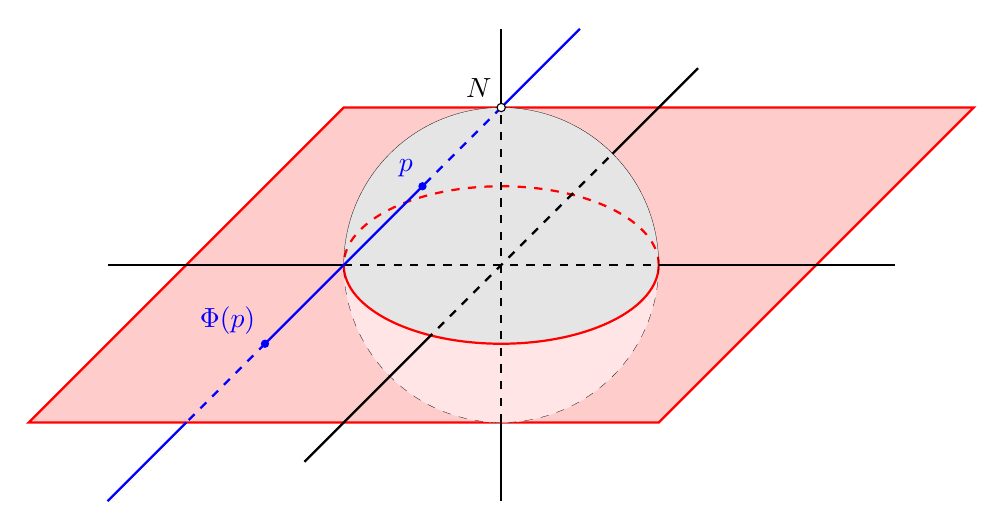
\begin{tikzpicture}

                % Plano
                \filldraw[thick, draw=red, fill=red!20] (-6,-2) -- (2,-2) -- (6,2) -- (-2,2) -- cycle;

                % Esfera principal
                \fill[line width=0.1pt, fill=gray!20] (0,0) circle (2cm);
                % \filldraw[fill=red!20, draw=red] (-3.5,-1.5) -- (2,-1.5) -- (4, 1) -- (-1.5, 1) --cycle; 
                
                \draw[red, thick, dashed] (2,0) arc[start angle=0, end angle=180, x radius=2, y radius=1];

                \fill[red!10, thick] (-2,0) arc[start angle=180, end angle=360, x radius=2, y radius=1] -- (2,0) arc[start angle=360, end angle=180, x radius=2, y radius=2] -- cycle;
                % \draw[red, thick,] (0,0) ellipse (2 and 1);

                % Parte inferior de la elipse
                \draw[red, thick] (-2,0) arc[start angle=180, end angle=360, x radius=2, y radius=1];

                % Contorno circunferencia
                \draw[line width=0.1pt, dashed](2,0) arc[start angle=360, end angle=180, x radius=2, y radius=2];
                \draw[line width=0.1pt](2,0) arc[start angle=0, end angle=180, x radius=2, y radius=2];

                % Eje vertical
                \draw[thick, dashed] (0,-2) -- (0,2);
                \draw[thick] (0,2) -- (0,3);
                \draw[thick] (0,-2) -- (0,-3);

                % Eje horizontal
                \draw[thick, dashed] (-2,0) -- (2,0);
                \draw[thick] (2,0) -- (5,0);
                \draw[thick] (-2,0) -- (-5,0);
                
                % Eje oblícuo
                \def\longitud{1.4142}
                \def\longitudd{0.95}
                \draw[thick, dashed] (-\longitudd,-\longitudd) -- (\longitud,\longitud);
                \draw[thick] (-2.5,-2.5) -- (-\longitudd,-\longitudd);
                \draw[thick] (\longitud,\longitud) -- (2.5,2.5);
                
                % Recta
                \draw[blue, thick] (1,3) -- (0,2);
                \draw[dashed, blue, thick] (0,2) -- (-1,1);
                \draw[blue, thick] (-1,1) -- (-3,-1);
                \draw[dashed, blue, thick] (-3,-1) -- (-4,-2);
                \draw[blue, thick] (-4,-2) -- (-5,-3);

                % Polo norte
                \filldraw[fill=white] (0,2) circle (1.5pt) node[above left]{$N$};

                % Punto p
                \fill[fill=blue] (-1,1) circle (1.5pt) node [above left] {\textcolor{blue}{$p$}};

                % Punto \Phi(p)
                \fill[fill=blue] (-3,-1) circle (1.5pt) node [above left] {\textcolor{blue}{$\Phi(p)$}};


            \end{tikzpicture}
        \end{center}

        Su inversa es 
        \begin{align*}
            \Phi^{-1}: \bb{R}^n &\to \bb{S}^n \setminus \{N\}\subset \bb{R}^{n+1}\\
            (y_1, \dots, y_n) & \mapsto \frac{1}{\|y\|^2+1}(2y_1, \dots, 2y_n, \|y\|^2-1)
        \end{align*}

        Tenemos que la aplicación 
        \begin{align*}
            \Phi:(\bb{S}^n\setminus \{N\}, \cc{T}_{|\bb{S}^n\setminus \{S\}}) \to (\bb{R}^n, \cc{T}_u)
        \end{align*}
        es un homeomorfismo ya que, como estamos en la topología usual podemos usar la intuición del análisis y ver que tanto $\Phi$ como $\Phi^{-1}$ son continuas y es fácil ver que $\Phi \circ \Phi^{-1} = Id_{\bb{S}^n\setminus \{N\}}$.

        Esta proyección se usa para hacer mapas de la Tierra, y por eso se producen deformaciones en la representación del mapa mundi. Hay mejores proyecciones para esto. Veamos la que viene a continuación:

        \item \textbf{Proyección de Mercator:} Esta proyección prueba que si se retiran 2 puntos de la esfera, el norte y el sur, la figura resultante es homeomorfa a un cilindro. Para ello se toma el punto central de la circunferencia y se proyecta una recta sobre los puntos $p$ de la esfera sin los polos. La intersección de dicha recta con el cilindro que tiene el radio de la esfera será $\varphi(p)$ y repitiendo esto en todos los puntos de la esfera obtenemos el cilindro de radio 1.
        
        %TODO: dibujo
        
        
        Sea $\bb{S}^n \subset \bb{R}^{n+1}$ la misma esfera definida en el apartado anterior y $S=(0,\dots, 0,-1)$ el polo sur. Podemos definir la siguiente aplicación:
        \begin{align*}
            \varphi : \bb{S}^n\setminus \{N, S\} &\to \bb{S}^{n-1}\times \bb{R}\\
            (x_1, \dots, x_n, x_{n+1}) &\mapsto \frac{1}{\|x\|} (x_1, \dots, x_n, x_{n+1})
        \end{align*}

        Esta aplicación es biyectiva y su inversa es
        \begin{align*}
            \varphi^{-1} : \bb{S}^{n-1}\times \bb{R} &\to \bb{S}^n \setminus \{N,S\}\\
            y=(y_1, \dots, y_n, y_{n+1}) &\mapsto \frac{y}{\|y\|}
        \end{align*}

        Es fácil ver que al componer ambas aplicaciones obtenemos la identidad. Con esta aplicación tenemos
        \begin{gather*}
            \varphi : (\bb{S}^n\setminus \{N,S\}, \cc{T}_{u_{|\bb{S}^n\setminus \{N,S\}}}) \to (\bb{S}^{n-1}\times \bb{R}, \cc{T}_{u_{|\bb{S}^{n-1}\times \bb{R}}})
        \end{gather*}
        es un homeomorfismo.
    \end{itemize}
    \endsquare
\end{ejemplo}

\begin{prop}
    Sea $f:(X, \cc{T})\to (Y, \cc{T}')$ un homeomorfismo. Entonces:
    \begin{enumerate}
        \item[(i)] Si $U\subset X$, entonces $U\in \cc{T}\sii f(U)\in \cc{T}'$.
        \item[(ii)] Si $C\subset X$, entonces $C\subset \cc{C}_{\cc{T}} \sii f(C)\in \cc{C}_{\cc{T}'}$.
        \item[(iii)] Si $\cc{B}\subset\cc{P}(X)$, entonces $\cc{B}$ es base de $\cc{T} \sii $ $\cc{B}'=f(B)=\{f(B):B\in \cc{B}\}$ es base de $\cc{T}'$.
        \item[(iv)] Si $x\in X$, y $N\in X$, entonces $N\in \cc{N}_x \sii f(N)\in \cc{N}_{f(x)}'$.
        \item[(v)] Si $x\in X$, $\cc{B}_x\subset \cc{P}(X)$, entonces $\cc{B}_x$ es b.d.e. de $x$ en $\cc{T} \sii \cc{B}_{f(x)}'=f(\cc{B}_x)=\{f(V):V\in \cc{B}_x\}$ es b.d.e. de $f(y)$ en $\cc{T}'$.     
    \end{enumerate}

    \begin{proof}
        Para las demostraciones veremos solo las implicaciones hacia la derecha ya que al ser un homeomorfismo, la implicación hacia la izquierda se basa en aplicar que $f^{-1}$ es también un homeomorfismo.

        \begin{enumerate}
            \item[(i)] Como $f$ es abierta se verifica.
            \item[(ii)] Como $f$ es cerrada se verifica.
            \item[(iii)] Tengo que comprobar varias cosas:
            \begin{itemize}
                \item $f(B)\in \cc{T}'$\ \ $\forall B \in base$. Esto es cierto ya que $B\in \cc{T}$ y $f$ es abierta.
                \item Sea $U'\in \cc{T}'$, $y\in U'$ tendré que ver que existe un abierto básico entremedias. Para ello tomo $f^{-1}(y)\subset f^{-1}(U')$ y como $f$ es continua tenemos que $f^{-1}(U')\in \cc{T}$. Como $\cc{B}$ es base tenemos que $\exists B \in \cc{B}$ con $f^{-1}(y)\in \cc{B}\subset f^{-1}(U')$ y como $f$ es biyectiva, $y\in f(B)\subset U'$ con $f(B)\in \cc{B}'$.
            \end{itemize}
            \begin{center}
                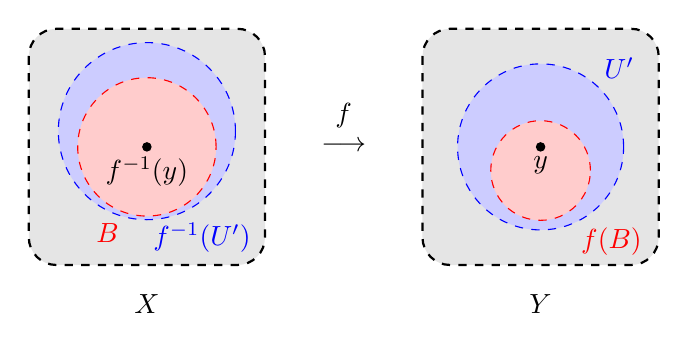
\begin{tikzpicture}
                    \def\incolor{gray!20}
        
                    \filldraw[rounded corners=10pt, dashed, thick, fill=\incolor] (0,0) rectangle (3,-3);
        
                    \node at (1.5, -3.5) {$X$};
                    \node at (4, -1.1) {$f$};
                    \node at (4, -1.5) {$\longrightarrow$};
        
                    \filldraw[rounded corners=10pt, dashed, thick, fill=\incolor] (5,0) rectangle (8,-3);
        
                    \node at (6.5, -3.5) {$Y$};
                    
                    \filldraw[dashed, draw=blue, fill=blue!20] (1.5, -1.3) circle (32pt);

                    \node at (2.2, -2.65) {\textcolor{blue}{$f^{-1}(U')$}};

                    \filldraw[dashed, draw=red, fill=red!20] (1.5, -1.5) circle (25pt);
        
                    \node at (1, -2.6) {\textcolor{red}{$B$}};
        
                    \filldraw[dashed, draw=blue, fill=blue!20] (6.5, -1.5) circle (30pt);
        
                    \filldraw[dashed, draw=red, fill=red!20] (6.5, -1.8) circle (18pt);
        
                    \node at (7.4, -2.7) {\textcolor{red}{$f(B)$}};
        
                    \node at (7.5, -0.5) {\textcolor{blue}{$U'$}};
        
                    \filldraw (1.5, -1.5) circle (1.5pt)  node[below] {$f^{-1}(y)$};
        
                    \filldraw (6.5, -1.5) circle (1.5pt)  node[below] {$y$};
        
                    
                \end{tikzpicture}
            \end{center}
            \item[(iv)] Sea $x\in X$, $N\in \cc{N}_x$. Como $\cc{N}_x$ es entorno, $\exists U\in \cc{T}$ con $x\in U\subset N' \Rightarrow f(x)\in f(U)\subset f(N)$ y como $f$ es abierta tengo que $f(U)\in \cc{T}'$ por lo que $f(N)\in \cc{N}_{f(x)}'$
            \item[(v)] Sea $N'\in \cc{N}_{f(x)}'$. Por (iv) (la implicación hacia la izquierda) tenemos que $f^{-1}(N')\in \cc{N}_x$. Como tenemos una b.d.e tenemos que $\exists V \in \cc{B}_x$ con $V\subset f^{-1}(N') \Rightarrow f(V)\subset N'$ y de nuevo por (iv) tenemos que $f(V)\in \cc{N}_{f(x)}'$ y tenemos lo que queríamos.
            \begin{center}
                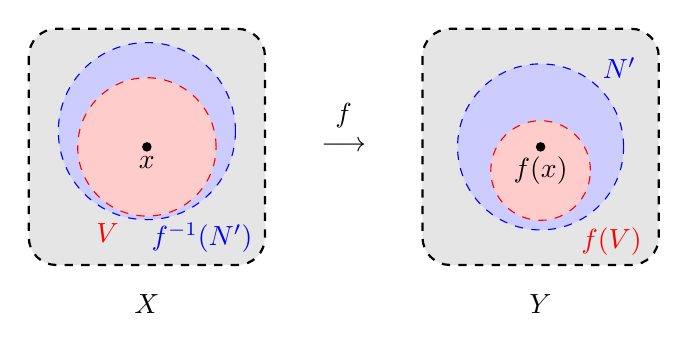
\begin{tikzpicture}
                    \def\incolor{gray!20}
        
                    \filldraw[rounded corners=10pt, dashed, thick, fill=\incolor] (0,0) rectangle (3,-3);
        
                    \node at (1.5, -3.5) {$X$};
                    \node at (4, -1.1) {$f$};
                    \node at (4, -1.5) {$\longrightarrow$};
        
                    \filldraw[rounded corners=10pt, dashed, thick, fill=\incolor] (5,0) rectangle (8,-3);
        
                    \node at (6.5, -3.5) {$Y$};
                    
                    \filldraw[dashed, draw=blue, fill=blue!20] (1.5, -1.3) circle (32pt);

                    \node at (2.2, -2.65) {\textcolor{blue}{$f^{-1}(N')$}};

                    \filldraw[dashed, draw=red, fill=red!20] (1.5, -1.5) circle (25pt);
        
                    \node at (1, -2.6) {\textcolor{red}{$V$}};
        
                    \filldraw[dashed, draw=blue, fill=blue!20] (6.5, -1.5) circle (30pt);
        
                    \filldraw[dashed, draw=red, fill=red!20] (6.5, -1.8) circle (18pt);
        
                    \node at (7.4, -2.7) {\textcolor{red}{$f(V)$}};
        
                    \node at (7.5, -0.5) {\textcolor{blue}{$N'$}};
        
                    \filldraw (1.5, -1.5) circle (1.5pt)  node[below] {$x$};
        
                    \filldraw (6.5, -1.5) circle (1.5pt)  node[below] {$f(x)$};
        
                    
                \end{tikzpicture}
            \end{center}
        \end{enumerate}
    \end{proof}
\end{prop}

\begin{definicion}
    Una propiedad $P$ que pueda o no tener un e.t. $(X, \cc{T})$ se dice \textbf{topológica} o que es un \textbf{invariante topológico} si al cumplirlo $(X, \cc{T})$, también la cumplen todos los espacios topológicos homeomorfos a él, es decir:
    \begin{gather*}
        (X, \cc{T}) \text{ cumple }P \sii (Y, \cc{T}') \text{ cumple } P\ \ \forall (Y, \cc{T}')\cong (X, \cc{T})
    \end{gather*}
    \endsquare
\end{definicion}

\begin{prop}
    Las propiedades \apuntar{T1}, \apuntar{T2}, \apuntar{1AN}, \apuntar{2AN} son invariantes topológicas.
    \begin{proof}
        Se deja como ejercicio para el lector %TODO: utilizar la proposición anterior (como la f es biyectiva son disjuntos)
    \end{proof}
\end{prop}

\begin{ejemplo}\
    \begin{itemize}
        \item $(\bb{R}, \cc{T}_u)\ncong (\bb{R}, \cc{T}_S)$ ya que $(\bb{R}, \cc{T}_u)$ es 2AN y $(\bb{R}, \cc{T}_S)$ no lo es.
        \item $(\bb{R}, \cc{T}_u)\ncong (\bb{R}, \cc{T}_{CF})\ncong (\bb{R}, \cc{T}_S)$ ya que $(\bb{R}, \cc{T}_u), (\bb{R}, \cc{T}_S)$ son T2 pero $(\bb{R}, \cc{T}_{CF})$ no lo es.
        \item $(\bb{R}, \cc{T}_u)\ncong (\bb{R}, \cc{T}_{disc})$ ya que $(\bb{R}, \cc{T}_{disc})$ no es 2AN.
    \end{itemize}
    \endsquare
\end{ejemplo}

\begin{definicion}
    Diremos que $f:(X, \cc{T})\to (Y, \cc{T}')$ es un \textbf{embebimiento} si $f^{f(X)}:(X, \cc{T})\to (f(X), \cc{T}_{f(X)}')$ es un homeomorfismo.
    En ese caso, $(X, \cc{T})\cong(f(X), \cc{T}_{f(X)}')$
    \endsquare
\end{definicion}

\begin{ejemplo}\
    \begin{itemize}
        \item $f$ homeomorfismo $\Rightarrow$ $f$ embebimiento. El recíproco no es cierto.
        \item Si $n, k \in \bb{N}$,
        \begin{align*}
            f:(\bb{R}^n, \cc{T}_u)&\to (\bb{R}^{n+k}, \cc{T}_u)\\
            x &\mapsto f(x)=(x,0)
        \end{align*}
        es un embebimiento con $f(\bb{R}^n)=\{\bb{R}^n \times \{0\}\}$.

        Para verlo tendremos que tomar la aplicación 
        \begin{align*}
            f^{\bb{R}^n\times \{0\}}:(\bb{R}^n, \cc{T}_u)&\to (\bb{R}^n\times \{0\}, \cc{T}_{u_{|\bb{R}^n\times \{0\}}})\\
            x &\mapsto (x,0)
        \end{align*}
        y tenemos además
        \begin{align*}
            (f^{\bb{R}^n\times \{0\}})^{-1}:(\bb{R}^n\times \{0\}, \cc{T}_{u_{|\bb{R}^n\times \{0\}}})&\to (\bb{R}^n, \cc{T}_u)\\
            (x,0) &\mapsto x
        \end{align*}
        y es fácil ver que $(f^{\bb{R}^n\times \{0\}})$ es un homeomorfismo y por tanto $f$ un embebimiento.
    \end{itemize}
    \endsquare
\end{ejemplo}

\section{Topología Producto}
En esta sección estudiaremos cómo a partir de dos e.t. $(X, \cc{T})$, $(Y, \cc{T}')$ podemos buscar una topología en el espacio $X\times Y$ a partir de $\cc{T}$ y $\cc{T}'$. Para ello, teniendo $X\times Y=\{(x,y):x\in X, y \in Y\}$ podemos tomar el conjunto $\{U\times U' : U\in \cc{T}, U'\in \cc{T}'\}$ pero vemos que no cumple la propiedad \apuntar{A2}. Sin embargo, sí podemos considerar que dicho conjunto sea una base de la topología producto.

\begin{prop}
    El conjunto 
    \begin{align*}
        \cc{B}_{\cc{T}\times \cc{T}'}=\{U\times U' : U\in \cc{T}, U'\in \cc{T}'\}
    \end{align*} 
    es base de una única topología en $X\times Y$ que se denota $\cc{T}\times \cc{T}'$ y se llama \textbf{topología producto} de $\cc{T}$ y $\cc{T}'$. 

    Al e.t. $(X\times Y, \cc{T}\times \cc{T}')$ lo llamaremos \textbf{espacio topológico producto} de $(X, \cc{T})$ y $(Y, \cc{T}')$.

    \begin{proof} Para ver que esto es cierto tendremos que comprobar que cumple las condiciones del Teorema \ref{teorema1_6}:
        \begin{enumerate}
            \item[\apuntar{B1}] $X\times Y \in \cc{B}_{\cc{T}\times \cc{T}'}\Rightarrow \bigcup\limits_{B\in \cc{B}_{\cc{T}\times \cc{T}'}}B=X\times Y$.
            \item[\apuntar{B2}] $U_1\times U_1', U_2\times U_2'\in \cc{B}_{\cc{T}\times \cc{T}'}$. Tenemos que $(U_1\times U_1')\cap (U_2\times U_2') = (U_1\cap U_2)\times (U_1'\times U_2')\in \cc{B}_{\cc{T}\times \cc{T}'}$. ya que $(U_1\cap U_2)\in \cc{T}$ y $(U_1'\cap U_2')\in \cc{T}'$.
        \end{enumerate}
        y ya lo tenemos probado.

    \end{proof}
\end{prop}

\begin{observacion}\
    \begin{itemize}
        \item Si $W\subset X\times Y$, entonces son equivalentes:
        \begin{enumerate}
            \item[(i)] $W\in \cc{T}\times \cc{T}'$.
            \item[(ii)] $\forall (x,y)\in W$\ \ $\exists U\in \cc{T}, U'\in \cc{T}'$ con $(x,y)\in U\times U'\subset W$.
            \item[(iii)] $\forall (x,y)\in W\ \ \exists U\in \cc{T}, U'\in \cc{T}'$ con $x\in U, y \in U', U\times U'\subset W$.
            \item[(iv)] $W=\bigcup\limits_{i\in I}(U_i\times U_i')$ con $U_i\in \cc{T}, U_i'\in \cc{T}'\ \ \forall i\in I$.
        \end{enumerate}
        \item En $(X\times Y, \cc{T}\times \cc{T}')$, todo producto de abiertos es abierto (básico) pero el recíproco no es cierto ya que hay abiertos en el producto que no son procducto de abiertos. Es decir, que la topología $\cc{T}\times \cc{T}'$ hay más abiertos en general que los básicos, es decir, $\cc{T}\times \cc{T}'\setminus \cc{B}_{\cc{T}\times \cc{T}'}\neq \emptyset$.
    \end{itemize}
\end{observacion}

\begin{prop}
    Sean $(X, \cc{T}), (Y, \cc{T}')$ dos e.t. Entonces:
    \begin{enumerate}
        \item[(i)] Si $\cc{B}$ es base de $\cc{T}$ y $\cc{B}'$ es base de $\cc{T}'$, entonces 
        \begin{align*}
            \tilde{\cc{B}}=\cc{B}\times \cc{B}'=\{B\times B': B\in \cc{B}, B'\in \cc{B}'\}
        \end{align*}
        es base de $\cc{T}\times \cc{T}'$.
        \item[(ii)] Si $x\in X$, $\cc{B}_x$ b.d.e. de $x$ en $(X, \cc{T})$ y $y\in Y$, $\cc{B}_y'$ b.d.e. de $y$ en $(Y, \cc{T}')$, entonces
        \begin{gather*}
            \tilde{\cc{B}}_{(x,y)}=\cc{B}_x\times \cc{B}_y' =\{V\times V': V\in \cc{B}_x, V'\in \cc{B}_y'\}
        \end{gather*}
        es b.d.e. de $(x,y)$ en $(X\times Y, \cc{T}\times \cc{T}')$.
    \end{enumerate}
    \begin{proof}\
        \begin{enumerate}
            \item[(i)] $\tilde{\cc{B}}=\cc{B}\times \cc{B}'\subset \cc{T}\times \cc{T}'$. Sea $W\in \cc{T}\times \cc{T}'$ y $(x,y)\in W$. Tendremos que ver que existe un elemento $B\times B'\in \tilde{\cc{B}}$ con $(x,y)\in B\times B'\subset W$. Como $\cc{B}_{\cc{T}\times \cc{T}'}$ es base de $\cc{T}\times \cc{T}'$, entonces $\exists U\in \cc{T}, U'\in \cc{T}'$ con $(x,y)\in U\times U'\subset W$. Como además $\cc{B}, \cc{B}'$ con bases tenemos que $\exists B\in \cc{B}, B'\in \cc{B}'$ con $x\in \cc{B}\subset U, y \in N'\subset U\Rightarrow (x,y)\in B\times B'\subset U\times U'\subset W$ y lo tenemos.
            \item[(ii)] La demostración es análoga a la anterior y se deja planteada como ejercicio para el lector.
        \end{enumerate}
    \end{proof}
\end{prop}

\begin{coro}
    $(X, \cc{T})$, $(Y, \cc{T})$ e.t.
    \begin{enumerate}
        \item[(i)] Si $(X, \cc{T})$ y $(Y, \cc{T}')$ son 1AN, entonces $(X\times Y, \cc{T}\times \cc{T}')$ es 1AN.
        \item[(ii)] Si $(X, \cc{T})$ y $(Y, \cc{T}')$ son 2AN, entonces $(X\times Y, \cc{T}\times \cc{T}')$ es 2AN.
    \end{enumerate}
    \endsquare
\end{coro}

\begin{ejemplo}\
    \begin{itemize}
        \item $\emptyset\neq A\subset X$, $\emptyset\neq A'\subset Y$ tenemos que $(\cc{T}, \cc{T}')_{|A\times A'}=\cc{T}_A \times \cc{T}_{A'}'$ (es fácil de comprobar).
        \item $\cc{T}_t\times \cc{T}_t = \cc{T}_t$.
        \item $\cc{T}_{disc}\times \cc{T}_{disc}=\cc{T}_{disc}$.
        \item $(\bb{R}^n\times \bb{R}^m, \cc{T}_u^n\times \cc{T}_u^m) = (\bb{R}^{n+m}, \cc{T}_u^{n+m})$.
        
        $B_{\infty}^n(x, \veps)\times B_{\infty}^m(y, \veps) = B_{\infty}^{n+m}((x,y), \veps)$.
    \end{itemize}
    \endsquare
\end{ejemplo}

\begin{observacion}
    Sean $(X, \cc{T})$, $(Y, \cc{T}')$ dos e.t., $C\in \cc{C}_{\cc{T}}$, $C'\in \cc{C}_{\cc{T}'}\Rightarrow C\times C'\in \cc{C}_{\cc{T}\times \cc{T}'}$.

    \begin{proof}
    En efecto, 
    \begin{gather*}
        (X\times Y)\setminus (C\times C')=\{(x,y)\in X\times Y : (x,y\notin C\times C')\} = ((X\setminus C \times Y)) \cup (X\times (T\setminus C'))
    \end{gather*}
    y como $((X\setminus C \times Y)), (X\times (T\setminus C')) \in \cc{T}\times \cc{T}'$, entonces la unión de abiertos en la topología producto es abierto. 
    
    \end{proof}

    Cabe destacar que el recíproco no es cierto, es decir, no todo cerrado en $\cc{T}\times \cc{T}'$ es producto de cerrados. Por ejemplo, en $(\bb{R}^2, \cc{T}_u)$, $([0,1]\times [0,1])\cup ([1,2] \times [1,2])$.

    \endsquare
\end{observacion}

\begin{definicion}
    Sean $X$, $Y$ dos conjuntos no vacíos, se definen las \textbf{proyecciones}
    \begin{align*}
        \pi_X:X\times Y &\to X \hspace*{1cm} &\pi_Y:X\times Y &\to Y\\
        (x,y) &\mapsto x  \hspace{1cm} &(x,y) &\mapsto y
    \end{align*}
    Son sobreyectivas
    \endsquare
\end{definicion}

\begin{prop}
    Sean $(X, \cc{T})$, $(Y, \cc{T}')$ e.t., entonces $\pi_X:(X\times Y, \cc{T}\times \cc{T}')\to (X, \cc{T})$ y $\pi_Y:(X\times Y, \cc{T}\times \cc{T}')\to (Y, \cc{T}')$ son continuas y abiertas.
    \begin{proof}
        Veamos en primer lugar que $\pi_X$ es continua. Sea $U\in \cc{T}$ tendré que ver que $\pi_X^{-1}(U)\in \cc{T}\times \cc{T}'$. Tenemos que $\pi_X^{-1}(U) = \{(x,y\in X\times Y : x\in U)\} = U\times Y \in \cc{T}\times \cc{T}'$.\\

        Veamos ahora que es abierta. Para ello consideramos $\cc{B}_{\cc{T}\times \cc{T}'}=\{U\times U' : U \in \cc{T}, U'\in \cc{T}'\}$ base de $\cc{T}\times \cc{T}'$. Sea $U\times U'\in \cc{B}_{\cc{T}\times \cc{T}'}$, entonces $\pi_X(U\times U')=U\in \cc{T}$.

    \end{proof}
\end{prop}

\begin{ejercicio}
    En general, las proyecciones no son cerradas.
    \endsquare
\end{ejercicio}

\begin{prop}
    Sean $(X, \cc{T})$, $(Y, \cc{T}')$ dos e.t., entonces $\cc{T}\times \cc{T}'$ es la topología menos fina en $X\times Y$ que hace que las proyecciones sean continuas. Es decir, si $\tilde{\cc{T}}$ es una topología en $X\times Y$ tal que $\pi_X:(X\times Y, \tilde{\cc{T}})\to (X, \cc{T})$ y $\pi_Y:(X\times Y, \tilde{\cc{T}})\to (Y, \cc{T}')$ son continuas, entonces $\cc{T}\times \cc{T}'\leq \tilde{\cc{T}}$.
    \begin{proof}
        Supongamos $\tilde{\cc{T}}$ y sea $U\times U'\in \cc{B}_{\cc{T}\times \cc{T}'}\Rightarrow U\in \cc{T}, U'\in \cc{T}'$. Tendremos que comprobar que $U\times U'\in \tilde{\cc{T}}$. Tenemos que
        \begin{align*}
            U\times U' &= \{(x,y)\in X\times Y : x\in U, y \in U'\} \\
            &= \{(x,y)\in X\times Y : x\in U\} \cap \{(x,y)\in X\times Y :y\in U'\} \\
            &= (U \times Y) \cap (X\times U') = \pi_X^{-1}(U) \cap \pi_Y^{-1}(U')
        \end{align*}
        Como $\pi_X$ y $\pi_Y$ son continuas, tenemos que $\pi_X^{-1}(U)\in \tilde{\cc{T}}$ y $\pi_Y^{-1}(U')\in \tilde{\cc{T}}$ por lo que su intersección también está en $\tilde{\cc{T}}$ y por tanto $U\times U'\in \tilde{\cc{T}}$.

    \end{proof}
\end{prop}

\begin{prop}(Placas del producto)\ 

    Sean $(X, \cc{T})$, $(Y, \cc{T}')$ dos e.t., $x_0\in X$, $y_0\in Y$, entonces
    \begin{align*}
        (X\times \{y_0\}, (\cc{T}\times \cc{T}')|_{X\times\{y_0\}})\cong (X, \cc{T})\\
        (\{x_0\}\times Y, (\cc{T}\times \cc{T}')|_{\{x_0\}\times Y})\cong (Y, \cc{T}')
    \end{align*}

    \begin{proof}
        Sea $\pi_{X_{|_{X\times \{y_0\}}}}$ y tenemos
        \begin{align*}
            (X\times \{y_0\}, (\cc{T}\times \cc{T}')_{X\times \{y_0\}}) &\to (X, \cc{T})\\
            (x,y_0) &\mapsto x
        \end{align*}
        Para ver que es un homeomorfismo tendremos que ver que es biyectiva (que es claro ya que su inversa sería la aplicación que lleva $x$ al par $(x,y_0)$), continua (que es claro por ser la restricción de una aplicación continua) y abierta. Veamos entonces que es abierta.

        Sea $\cc{B}_{\cc{T}\times \cc{T}'}=\{U\times U': U\in \cc{T}, U'\in \cc{T}'\}$ base de $\cc{T}\times \cc{T}'$. Consideramos $\cc{B}=\{(U\times U')\cap (X\times \{y_0\}): U\in \cc{T}, U'\in \cc{T}'\}$ que es base del subespacio. Tenemos entonces:
        
        \begin{align*}
            A=(U\times U')\cap (x\times \{y_0\}) = \left\{
            \begin{array}{lcc}
                \emptyset & \text{ si } & y_0\notin U'\\
                U\times \{y_0\} & \text{ si } & y_0\in U'\\
            \end{array}
            \right.
        \end{align*}
        Tenemos que
        \begin{align*}
            \pi_{X_{|_{X\times\{y_0\}}}} (A) = \pi_X(A) = \left\{
                \begin{array}{lcc}
                    \emptyset & \text{ si } & y_0\notin U'\\
                    U & \text{ si } & y_0\in U'\\
                \end{array}
                \right.
        \end{align*}
        Por lo que $\pi_{X_{|_{X\times\{y_0\}}}} (A)\in \cc{T}$ y ya tenemos que es abierta y por tanto un homeomorfismo.
    \end{proof}
\end{prop}

\begin{prop}
    Sean $(X, \cc{T})$, $(Y, \cc{T}')$ dos e.t., entonces
    \begin{enumerate}
        \item[(i)] $(X\times Y, \cc{T}\times \cc{T}')$ es 1AN $\sii (X, \cc{T})$ y $(Y, \cc{T}')$ son 1AN.
        \item[(ii)] $(X\times Y, \cc{T}\times \cc{T}')$ es 2AN $\sii (X, \cc{T})$ y $(Y, \cc{T}')$ son 2AN.
        \item[(iii)] $(X\times Y, \cc{T}\times \cc{T}')$ es T1 $\sii (X, \cc{T})$ y $(Y, \cc{T}')$ son T1. 
        \item[(iv)] $(X\times Y, \cc{T}\times \cc{T}')$ es T2 $\sii (X, \cc{T})$ y $(Y, \cc{T}')$ son T2.
        \item[(v)] $(X\times Y, \cc{T}\times \cc{T}')$ es metrizable $\sii (X, \cc{T})$ y $(Y, \cc{T}')$ son metrizables.
    \end{enumerate}
    \begin{proof}\
        \begin{itemize}
            \item[$\Rightarrow)$] Supongamos que $(X\times Y, \cc{T}\times \cc{T}')$ cumple $P$, entonces $(X\times\{y_0\}, (\cc{T}\times \cc{T}')_{X\times\{x_0\}})$ cumple $P$ y como $P$ es un invariante topológico, entonces $(X, \cc{T})$ que es homeomorfo a dicho espacio también la cumple. Análogamente obtengo que $(Y, \cc{T}')$ también verifica $P$ (considerando el subespacio $(\{x_0\}\times Y, (\cc{T}\times \cc{T}')_{\{x_0\}\times Y})$).
            \item[$\Leftarrow)$] 
            \begin{itemize}
                \item[(i)] Hecho en clase.
                \item[(ii)] Hecho en clase
                \item[(iii)] Es análoga que (iv)
                \item[(iv)] Sean $(x,y), (x', y')\in X\times Y$ con $(x,y)\neq (x',y')$ y supongamos que $x\neq x'$ (esto no quita generalidad ya que en caso de que $x=x'$, entonces necesariamente $y\neq y'$ y se razonaría de forma simétrica). Como $X$ es T2, entonces existen $U_1, U_2\in \cc{T}$ con $x\in U_1$, $x'\in U_2$ y $U_1 \cap U_2 = \emptyset \Rightarrow (x,y)\in U_1 \times Y \in \cc{T}\times \cc{T}'$ y $(x',y')\in U_2 \times Y\in \cc{T}\times \cc{T}'$ por lo que tenemos que $(U_1\times Y)\cap (U_2\times Y) = (U_1 \cap U_2)\times Y = \emptyset \times Y = \emptyset$ y lo tenemos.
                \item[(v)] Es un ejercicio de análisis I. Se hace de la siguiente forma. Supongamos que $\cc{T}=\cc{T}_d$ y $\cc{T}'=\cc{T}_{d'}$ y podemos definir
                \begin{align*}
                    \tilde{d} :(X\times Y) &\to [0,+\infty]\\
                    ((x,y),(x',y')) & \mapsto d(x,x') + d'(y,y')
                \end{align*}
                Solo quedaría comprobar que $\tilde{d}$ es una distancia en $X\times Y$ (que no es materia de esta asignatura) y comprobar que $\cc{T}_{\tilde{d}} = \cc{T}\times \cc{T}'$.
            \end{itemize}
        \end{itemize}
    \end{proof}
\end{prop}

\begin{definicion}
    Sea $f:Z \to X \times Y$ una aplicación, escribimos $f=(f_X, f_Y)$ donde
    \begin{align*}
        f_X=\pi_X \circ f: Z \to X\\
        f_Y=\pi_Y \circ f: Z \to Y
    \end{align*}
    A estas aplicaciones las llamaremos \textbf{aplicaciones componentes} de $f$. Tenemos entonces $f(z)=(f_X(z), f_Y(z))\in (X \times Y)$.
    \endsquare
\end{definicion}

\begin{prop}
    Sean $(X, \cc{T})$, $(Y, \cc{T}')$ y $(Z, \cc{T}'')$ e.t. Si $f:(Z, \cc{T}'')\to (X\times Y, \cc{T}\times \cc{T}')$ es una aplicación, entonces:
    \begin{align*}
        f \text{ es continua } \sii 
        \begin{array}{c}
            f_X=\pi_X \circ f : (Z, \cc{T}'')\to (X, \cc{T})\\
            f_Y=\pi_Y \circ f : (Z, \cc{T}'')\to (Y, \cc{T}')\\
        \end{array}
        \text{ son continuas}
    \end{align*}
    Es decir, la función $f$ es continua si y solo si lo es en cada una de sus componentes.
    \begin{proof}\
        \begin{itemize}
            \item[$\Leftarrow$)] Trivial por ser composición de aplicaciones continuas.
            \item[$\Rightarrow$)] Sea $U\times U'\in \cc{B}_{\cc{T}\times \cc{T}'}\subset \cc{T}\times \cc{T}'$. Tendremos que ver que $f^{-1}(U\times U')\in \cc{T}''$. Veamos cuál es la imagen inversa. Tenemos que
            \begin{align*}
                f^{-1}(U\times U') &= \{z\in Z : f(z)\in (U\times U')\} = \{z \in Z : f_X(z)\in U, f_Y(z)\in U'\}=\\
                &= f_X^{-1}(U)\cap f_Y^{-1}(U')\in \cc{T}''
            \end{align*}
            por ser intersección de abiertos en $\cc{T}''$.
        \end{itemize}
    \end{proof}
\end{prop}

\begin{definicion}
    Sean $X_1, X_2, Y_1, Y_2\neq \emptyset$, $f_1:X_1 \to Y_1$, $f_2:X_2 \to Y_2$ aplicaciones, se define la \textbf{aplicación producto} de $f_1$ y $f_2$ como
    \begin{align*}
        f_1 \times f_2 : X_1 \times X_2 &\to Y_1 \times Y_2\\
        (x_1, x_2) &\mapsto (f_1 \times f_2)(x_1, x_2) = (f_1(x_1), f_2(x_2))
    \end{align*}
    \endsquare
\end{definicion}

\begin{prop}
    Sean $(X_i, \cc{T}_i)$, $(Y_i, T_i')$ e.t. para $i=1,2$ y $f_i(X_i, \cc{T}_i)\to (Y_i, \cc{T}_i')$ funciones entre e.t. para $i=1,2$. Consideramos la aplicación producto $f_1\times f_2:(X_1 \times X_2, \cc{T}_1 \times \cc{T}_2)\to (Y_1 \times Y_2, \cc{T}_1' \times \cc{T}_2')$. Entonces 
    \begin{enumerate}
        \item[(i)] $f_1 \times f_2$ es continua $\sii$ $f_1$ y $f_2$ son continuas.
        \item[(ii)] $f_1 \times f_2$ es abierta $\sii$ $f_1$ y $f_2$ son abiertas.
        \item[(iii)] $f_1 \times f_2$ es homeomorfismo $\sii$ $f_1$ y $f_2$ son homeomorfismos.
    \end{enumerate}
    \begin{proof}\
        \begin{enumerate}
            \item[(i)] Sea $ U_1'\times U_2 '\in \cc{B}_{\cc{T}_1'\times \cc{T}_2'} \Rightarrow (f_1 \times f_2)^{-1}(U_1'\times U_2')=f_1^{-1}(U_1')\times f_2^{-1}(U_2')$
            \begin{itemize}
                \item[$\Rightarrow$)] $f_1^{-1}(U_1') \times f_2^{-1}(U_2')\in \cc{T}_1 \times \cc{T}_2$. Como la proyección $\pi_{X_1}$ es abierta, $\pi_{X_1}(f_1^{-1}(U_1') \times f_2^{-1}(U_2'))=f_1^{-1}(U_1')$ 
                \item[$\Leftarrow$)] Trivial 
            \end{itemize}
            \item[(ii)] $(f_1 \times f_2)(U_1\times U_2)=f_1(U_1)\times f_2(U_2)$.
            \item[(iii)] $(f_1\times f_2)^{-1}=f_1^{-1}\times f_2^{-1}$ 
        \end{enumerate}
    \end{proof}
\end{prop}

\begin{coro}
    Si $(X_i, \cc{T}_i) \cong (Y_i, \cc{T}_i')$ con $i=1,2$, entonces:
    \begin{align*}
        (X_1 \times X_2, \cc{T}_1 \times \cc{T}_2) \cong (Y_1 \times T_2, \cc{T}_1'\times \cc{T}_2')
    \end{align*}
    \endsquare
\end{coro}

\begin{definicion}
    (Productos finitos) Sean $(X_i, \cc{T}_i)$ e.t. para $i=1,\dots,n$ con $n\in \bb{N}$, definimos:
    \begin{align*}
        \cc{B}_{\cc{T}_1 \times \dots \times \cc{T}_n}= \{U_1 \times U_2 \times \dots \times U_n : U_i \in \cc{T}_i\ \ \forall i \in\{1,\dots,n\} \} \subset \cc{P}(X_1 \times \dots \times X_n)
    \end{align*}
    Entonces $\cc{B}_{\cc{T}_1 \times \dots \times \cc{T}_n}$ es base de una única topología $\cc{T}_1, \dots, \cc{T}_n$ en $X_1, \dots, X_n$. Al espacio topológico $(X_1\times \dots \times X_n, \cc{T}_1 \times \dots \times \cc{T}_n)$ lo llamaremos \textbf{espacio topológico producto} de $(X_i, \cc{T}_i)$
    \endsquare
\end{definicion}

\begin{observacion}
    Todos los resultados vistos para $n=2$ son ciertos para cualquier $n\geq 2$.
    \endsquare
\end{observacion}

\begin{definicion}
    (Topología inicial) Sean $X\neq \emptyset$ un conjunto, $\{(X_i, \cc{T}_i)\}_{i\in I}$ una familia de e.t. y $\cc{F}=\{f_i:X \to X_i\}_{i\in I}$ una familia de aplicaciones. Se llama \textbf{topología inicial} en $X$ para la familia $\cc{F}$ a la única topología $\cc{T}_{\cc{F}}$ que tiene por subbase a 
    \begin{gather*}
        \emptyset \neq S = \{f^{-1}(U_i) : U_i \in X_i, i\in I\} \subset \cc{P}(X)
    \end{gather*}
    \endsquare
\end{definicion}

\begin{prop}
    Con esta notación:
    \begin{enumerate}
        \item[(i)] $f_i:(X, \cc{T}_{\cc{F}}) \to (X_i, \cc{T}_i)$ es continua $\forall i \in I$.
        \item[(ii)] Si $\cc{T}$ es una topología en $X$ y $f_i:(X, \cc{T})\to (Y_i, \cc{T}_i)$ es continua $\forall i\in I$, entonces $\cc{T}_{\cc{F}}\leq \cc{T}$
        \item[(iii)] Si $f:(Z, \cc{T}')\to (X, \cc{T}_{\cc{F}})$, entonces $f$ es continua $\sii (f_i\circ f)(Z, \cc{T}') \to (X_i, \cc{T}_i)$ es continua $\forall i \in I$
    \end{enumerate}
    \begin{proof}\
        \begin{enumerate}
            \item[(i)] Trivial
            \item[(ii)] Trivial
            \item[(iii)] Se deja planteada como ejercicio para el lector %TODO  
        \end{enumerate}
    \end{proof}
\end{prop}

\begin{ejemplo}\
    \begin{itemize}
        \item Si $(X, \cc{T})$, $Y, \cc{T}'$ son e.t. y $\cc{F}=\{\pi_X: X\times Y \to X, \pi_Y:X\times Y \to Y\}$, entonces $(X\times Y, \cc{T}_{\cc{F}}) = (X\times Y, \cc{T}\times \cc{T}')$
        \item Si $(X, \cc{T})$ e.t., $\emptyset \neq A \subset X$, $\cc{F}=\{i_A: A\to X\}$ (donde $i_A$ es la aplicación inclusión de $A$), entonces $(A, \cc{T}_{\cc{F}})=(A, \cc{T}_A)$ (ya que $i_A^{-1}(U)=U \cap A$).
    \end{itemize}
\end{ejemplo}

\section{Identificaciones y topología cociente}

\begin{teo}
    Sea $(X, \cc{T})$ un e.t., $Y\neq \emptyset$ un conjunto y la aplicación $f:(X, \cc{T})\to Y$, entonces la familia
    \begin{gather*}
        \cc{T}_f = \{U'\subset Y : f^{-1}(U')\in \cc{T}\}\subset \cc{P}(Y)
    \end{gather*}
    es una topología en $Y$ que llamamos \textbf{topología final} para la aplicación $f$. Además,
    \begin{enumerate}
        \item[(i)] $f:(X, \cc{T})\to (Y, \cc{T}_f)$ es continua.
        \item[(ii)] Si $\cc{T}'$ es una topología en $Y$ con $f:(X, \cc{T})\to (Y, \cc{T}')$ es continua, entonces $\cc{T}'\leq \cc{T}_f$
    \end{enumerate}
    \begin{proof}
        Veamos en primer lugar que efectivamente $\cc{T}_f$ es una topología en $X$
        \begin{enumerate}
            \item[\apuntar{A1}] $f^{-1}(\emptyset)=\emptyset \in \cc{T} \Rightarrow \emptyset\in \cc{T}_f$. $f^{-1}(Y)=X\in \cc{T}\Rightarrow Y \in \cc{T}_f$
            \item[\apuntar{A2}] Sea $\{U_i'\}_{i\in I}\subset \cc{T}_f$. Queremos ver que $\bigcup\limits_{i\in I}U_i'\in \cc{T}_f$.
            \begin{gather*}
                f^{-1}\left(\bigcup\limits_{i\in I}U_i'\right) = \bigcup\limits_{i\in I} f^{-1}(U_i')\in \cc{T} \Rightarrow \bigcup\limits_{i\in I}U_i'\in \cc{T}_f
            \end{gather*}
            \item[\apuntar{A3}] Sean $U_1', U_2'\in \cc{T}_f$ tendremos que ver que $U_1'\cap U_2'\in \cc{T}_f$.
            \begin{gather*}
                f^{-1}(U_1'\cap U_2)=f^{-1}(U_1')\cap f^{-1}(U_2')\in \cc{T}
            \end{gather*}
            por ser intersección de abiertos en $\cc{T}$.
        \end{enumerate}
        Veamos ahora que verifica las 2 propiedades que menciona el teorema:
        \begin{enumerate}
            \item[(i)] Trivial (por la definición de $\cc{T}_f$)
            \item[(ii)] Sea $U'\in \cc{T}$ veamos que entonces $U'\in \cc{T}_f$. Por ser $f$ continua tenemos que $f^{-1}(U')\in \cc{T}\Rightarrow U'\in \cc{T}_f$ y lo tenemos probado.
        \end{enumerate}
    \end{proof}
\end{teo}

\begin{ejemplo}\
    \begin{itemize}
        \item $Id_X:(X, \cc{T})\to X$. $\cc{T}_{Id_X}=\{U\in X : Id_X^{-1}(U) \in \cc{T}\}=\{U\in X : U \in \cc{T}\}$
        \item $f:(X, \cc{T})\to Y$ constante, es decir, $f(x)=y_0\in Y\ \ \forall x \in X$. Entonces tenemos que $\cc{T}_f=\cc{T}_{disc}$ ya que
        \begin{align*}
            \cc{T}_f=\{U'\subset Y : f^{-1}(U')\in \cc{T}\}=\cc{P}(Y)
        \end{align*}
        Esto se debe a que
        \begin{align*}
            f^{-1}(U')=\left\{
            \begin{array}{ccc}
                X & \text{ si } & y_0\in U'\\
                \emptyset & \text{ si } & y_0\notin U'
            \end{array}
            \right.
        \end{align*} 
        \item Consideramos la siguiente función
        \begin{align*}
            f:([0,1], \cc{T}_u|_{[0,1]})&\to Y=\{0,1\}\\
            x &\mapsto \left\{
            \begin{array}{ccc}
                1 & \text{ si } & x \in [0,\nicefrac{1}{2}]\\
                0 & \text{ si } & x \in (\nicefrac{1}{2}, 1]
            \end{array}
            \right.
        \end{align*}
        Entonces tenemos que
        \begin{align*}
            \cc{T}_f=\{U'\subset \{0,1\} : f^{-1}(U')\in \cc{T}_u|_{[0,1]}\}=\{\emptyset, \{0,1\}, \{0\}\}
        \end{align*}
        Veamos por qué $\{0\}\in \cc{T}_f$ pero $\{1\}\notin \cc{T}_f$
        \begin{align*}
            f^{-1}(\{0\})=(\nicefrac{1}{2},1] \in \cc{T}_u|_{[0,1]}\Rightarrow \{0\}\in \cc{T}_f\\
            f^{-1}(\{1\})=[0,\nicefrac{1}{2}] \notin \cc{T}_u|_{[0,1]}\Rightarrow \{1\}\notin \cc{T}_f\\
        \end{align*}
    \end{itemize}
    \endsquare
\end{ejemplo}

\begin{prop}
    Sea $f:(X,Y)\to Y$ una aplicación. Entonces:
    \begin{enumerate}
        \item[(i)] Una aplicación $g:(Y, \cc{T}_f)\to (Z, \cc{T}'')$ es continua si y solo si $g\circ f:(X, \cc{T})\to (Z, \cc{T}'')$ es continua.
        \begin{center}
            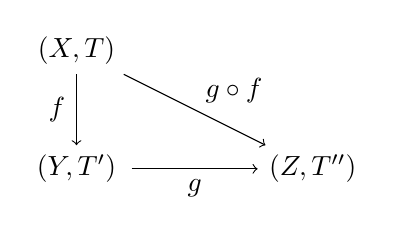
\begin{tikzpicture}
                % Desactiva los caracteres conflictivos
                \shorthandoff{>} % Para poner puntas de flecha

                \node at (0,0) {$(X, \cc{T})$};
                \node at (0,-1.5) {$(Y, \cc{T}')$};
                \node at (3,-1.5) {$(Z, \cc{T}'')$};

                \draw[->] (0.6,-0.3) -- (2.4,-1.2);
                \draw[->] (0,-0.3) -- (0,-1.2);
                \draw[->] (0.7,-1.5) -- (2.3,-1.5);

                \node at (2,-0.5) {$g\circ f$};
                \node at (-0.25, -0.75) {$f$};
                \node at (1.5, -1.75) {$g$};
            \end{tikzpicture}
        \end{center}
        \item[(ii)] $\cc{C}_{\cc{T}_f}=\{C'\subset Y : f^{-1}(C')\in \cc{C}_{\cc{T}}\}$
    \end{enumerate}
    \begin{proof}\
        \begin{enumerate}
            \item[(i)] 
            \begin{itemize}
                \item[$\Rightarrow$)] Por ser $g\circ f$ composición de continuas.
                \item[$\Leftarrow$)] Sea $U''\in \cc{T}''$, tendremos que ver que $g^{-1}(U'')\in \cc{T}_f$.
                \begin{align*}
                    f^{-1}(g^{-1}(U'')) \overset{\ast}{=} (g\circ f)^{-1}(U'')\in \cc{T}\Rightarrow g^{-1}(U'')\in \cc{T}_f
                \end{align*}
                Donde en $\ast$ hemos tenido en cuenta que $g\circ f$ es continua. Por tanto tenemos que $g$ es continua.
            \end{itemize}
            \item[(ii)] Sea $C'\subset Y$, $C'\in \cc{C}_{\cc{T}_f}\sii Y\setminus C' \in \cc{T}_f \sii f^{-1}(Y\setminus C')\in \cc{T} \sii f^{-1}(C')\in \cc{C}_{\cc{T}}$
        \end{enumerate}
    \end{proof}
\end{prop}

\begin{definicion}
    Una aplicación $p:(X, \cc{T})\to (Y, \cc{T}')$ es una \textbf{identificación} si $p$ es sobreyectiva y $\cc{T}'=\cc{T}_p$.
    \endsquare
\end{definicion}

\begin{observacion}\
    \begin{itemize}
        \item Toda identificación es continua.
        \item Si $p:(X, \cc{T})\to (Y, \cc{T}')$ es una identificación y $g:(Y, \cc{T}')\to(Z, \cc{T}'')$ es otra aplicación con $\cc{T}'=\cc{T}_p$, entonces $g$ es continua $\sii g\circ p: (X, \cc{T})\to (Z, \cc{T}'')$ es continua.
    \end{itemize}
\end{observacion}

\begin{ejemplo}\
    \begin{itemize}
        \item $Id_X:(X, \cc{T})\to (X, \cc{T}')$ es identificación $\sii \cc{T}=\cc{T}'$.
        \item $p: \cc{X}_{[0,\nicefrac{1}{2})}:([0,1], \cc{T}_u|_{[0,1]})\to (\{0,1\}, \cc{T}_f=\{\emptyset, \{0,1\}, \{0\}\})$ es identificación pero no es abierta ni cerrada.
        \begin{align*}
            p([0,\nicefrac{1}{4})) = \{1\}\notin \cc{T}_f \text{ pero } [0,\nicefrac{1}{4})\in \cc{T}_u|_{[0,1]}\\
            p([\nicefrac{3}{4}, 1])=\{0\}\notin \cc{C}_{\cc{T}_p} \text{ pero } [\nicefrac{3}{4}, 1] \in \cc{C}_{\cc{T}_u\_{[0,1]}}
        \end{align*}
    \end{itemize}
    \endsquare
\end{ejemplo}

\begin{prop}
    Si $f:(X, \cc{T})\to (Y, \cc{T}')$ es continua, sobreyectiva y abierta, o continua, sobreyectiva y cerrada, entonces $f$ es una identificación.
    \begin{proof}
        Por hipótesis tenemos que $f$ es sobreyectiva y queremos ver que $\cc{T}'=\cc{T}_f$. Como $f$ es continua tenemos que $\cc{T}'\leq \cc{T}_f$. Supongamos que $f$ es abierta y querremos ver la otra inclusión. Sea $U'\in \cc{T}_f$, entonces tenemos que $f^{-1}(U)\in \cc{T}$. Por ser $f$ abierta tenemos que $f(f^{-1}(U))\in \cc{T}'$ y ya tenemos probada la doble inclusión.\\

    \end{proof}
\end{prop}

\begin{observacion}
    Una identificación puede no ser abierta ni cerrada.
    \endsquare
\end{observacion}

%TODO: Lo último es descripción de los abiertos en la topología cociente

\begin{ejemplo}\
    $\pi_X(X\times Y, \cc{T}\times \cc{T}')\to (X, \cc{T})$ es una identificación
    \endsquare
\end{ejemplo}

\begin{coro}
    Sea $f:(X, \cc{T})\to (T, \cc{T})$ una aplicación. Entonces $f$ es un homeomorfismo si y solo si $f$ es una identificación inyectiva.
    \begin{proof}\
        \begin{itemize}
            \item[$\Rightarrow$)] Si $f$ es un homeomorfismo entonces por definición es inyectiva, sobreyectiva, continua y abierta por lo que es una identificación inyectiva.
            \item[$\Leftarrow$)] Si $f$ es una identificación inyectiva entonces, por definición es biyectiva, continua y $\cc{T}=\cc{T}_f$. Veamos que además es abierta. Para ello consideramos $U\in \cc{T}$ y tenemos que $f(U)\in \cc{T}_f \sii f^{-1}(f(U))\in \cc{T}$ lo cual se verifica por ser sobreyectiva. Como $f(U)\in \cc{T}_f$, entonces $f$ es abierta y por tanto es un homeomorfismo.
        \end{itemize}
    \end{proof}
\end{coro}

\begin{definicion}
    Si $p:X\to Y$ es una aplicación y $A\subset X$, diremos que $A$ es \textbf{p-saturado} si $p^{-1}(p(A))=A$, esto es, $p^{-1}(p(A))\subset A$ (la otra inclusión siempre se da).
    \endsquare
\end{definicion}

\begin{prop}
    Sea $(X, \cc{T})$ un e.t., $Y$ un conjunto y $p:X\to Y$ una aplicación sobreyectiva. Entonces
    \begin{enumerate}
        \item[(i)] $\cc{T}_p=\{p(U):U\in \cc{T} \text{ con } U \text{ p-saturado}\}$
        \item[(ii)]  $\cc{C}_{\cc{T}_p}=\{p(C):C\in \cc{C}_{\cc{T}} \text{ con } C \text{ p-saturado}\}$
    \end{enumerate}
    \begin{proof}\
        \begin{itemize}
            \item[(i)] Veámoslo por doble inclusión:
            \begin{itemize}
                \item[$\subseteq$)] Sea $U'\in \cc{T}_p$, entonces $p^{-1}(U')\in \cc{T}$. Si tomo $U=p^{-1}(U')$ tendremos que ver que $U$ es p-saturado. Tenemos que $p^{-1}(p(U))=p^{-1}(p(p^{-1}(U')))=p^{-1}(U')=U$ y lo tenemos.
                \item[$\supseteq$)] Sea $U\in \cc{T}$ con $p^{-1}(p(U))=U$ tendremos que ver que $p(U)\in \cc{T}_p$. Por ser $U$ p-saturado tenemos que $p^{-1}(p(U))=U\in \cc{T}\in \cc{T}$.
            \end{itemize}
            \item[(ii)] Se deja planteada como ejercicio para el lector.
        \end{itemize}
    \end{proof}
\end{prop}

\begin{coro}
    Si $p:(X, \cc{T})\to (Y, \cc{T}')$ es una aplicación sobreyectiva, entonces equivalen:
    \begin{enumerate}
        \item[(i)] $p$ es una identificación.
        \item[(ii)] $\cc{T}'=\cc{T}_p=\{p(U):U\in \cc{T} \text{ p-saturado}\}$.
        \item[(iii)] $\cc{C}_{\cc{T}'}=\cc{C}_{\cc{T}_p}=\{p(C):C\in \cc{C}_{\cc{T}} \text{ p-saturado}\}$. 
    \end{enumerate}
    \endsquare
\end{coro}

\begin{prop}
    Sean $p:(X, \cc{T}) \to (Y, \cc{T}')$ y $p':(Y, \cc{T}') \to (Z, \cc{T}'')$ aplicaciones y consideramos su composición $p'\circ p:(X, \cc{T})\to (Z, \cc{T}'')$. Entonces:
    \begin{enumerate}
        \item[(i)] $p,p'$ identificaciones $\Rightarrow$ $p'\circ p$ identificación.
        \item[(i)] $p,p'$ continuas y $p'\circ p$ identificación $\Rightarrow p'$ identificación.
        \item[(iii)] $p$ identificación $\Rightarrow$ ($p'$ identificación $ \sii p'\circ p$ identificación). 
    \end{enumerate}
    \begin{proof}\ 
        La demostración se deja planteada como ejercicio para el lector.

    \end{proof}
\end{prop}

\begin{coro}
    Si $p:(X, \cc{T})\to (Y, \cc{T}')$ continua y admite una inversa continua por la derecha, es decir, $\exists f:(Y, \cc{T}')\to (X, \cc{T})$ continua y tal que $p\circ f=Id_Y$, entonces $p$ es una identificación.
    \begin{proof}
        Como $p\circ f=Id_Y$ es un homeomorfismo, en particular es una identificación y como $f$ y $p$ son continuas, por la proposición anterior sabemos que $p$ es una identificación. 

    \end{proof}
\end{coro}

\begin{definicion}
    Sea $(X, \cc{T})$ un e.t. y sea $R$ una relación de equivalencia en $X$ con la proyección dada por
    \begin{align*}
        p:X&\to X/R\\
        x &\mapsto [x] = \{x'\in X : xRx'\}
    \end{align*}
    Llamaremos \textbf{topología cociente} y la notaremos por $T/R$ a la topología final en $X/R$ asociada a $p$, esto es $T/R=T_p$. Al espacio topológico $(X/R, \cc{T}/R)$ se le llama \textbf{espacio topológico cociente} de $(X, \cc{T})$ por la relación de equivalencia $R$.
    \endsquare
\end{definicion}

\begin{propiedades}
    En esta situación, $p:(X, \cc{T})\to (X/R, \cc{T}/R)$ es una identifiación, luego:
    \begin{enumerate}
        \item[(i)] $p$ es continua y $T/R$ es la topología más fina que hace a $p$ continua.
        \item[(ii)] $f:(X/R, \cc{T}/R)\to (Y, \cc{T}')$ continua $\sii f\circ p:(X, \cc{T})\to (Y, \cc{T}')$ continua.
        \item[(iii)] $\cc{T}/R=\{\tilde{U}\subset X/R : p^{-1}(\tilde{U})\in \cc{T}\} = \{p(U) : U\in \cc{T} \text{ p-saturado}\}$.
        \item[(iv)] $\cc{C}_{\cc{T}/R} = \{\tilde{C}\subset X/R : p^{-1}(\tilde{C})\in \cc{C}_{\cc{T}}\} = \{p(C) : C\in \cc{C}_{\cc{T}} \text{ p-saturado}\}$.
        \item[(v)] $A\subset X$ es p-saturado $\sii p^{-1}(p(A))=A \sii p(a)=[a]\subset A\ \ \forall a \in A \sii x\in A\ \ \forall x\in X$ tal que $\exists a \in A$ con $xRa$.
    \end{enumerate}
    \endsquare
\end{propiedades}

\begin{definicion}
    Si $f:X \to Y$ es una aplicación y $R$ es una relación de equivalencia en $X$ con proyección $p:X \to X/R$.
    %      f
    %   X ---> Y
    % P |   / (discontinua y flecha hacia arriba)
    %   v  /  \tilde{f}
    %   X/R

    \begin{figure}[H]
        \centering
        \shorthandoff{""}
        \begin{tikzcd}
            X \arrow[d, "p"'] \arrow[r, "f"]    & Y \\
            X/R \arrow[ru, "\tilde{f}", dashed] &  
        \end{tikzcd}
        \shorthandon{""}
    \end{figure}
    

    Se dice que $f$ es \textbf{compatible} con $R$ si $f(x)=f(x')$\ \ $\forall x, x' \in X$ con $xRx'$. En este caso, la aplicación $f$ \textbf{baja al cociente} como una aplicación bien definida, es decir, que hace que el diagrama sea conmutativo. Se le suele notar por $\tilde{f}:X/R \to Y$ tal que $\tilde{f}([x]_R)=f(x)$ con $\tilde{f}\circ p = f$.
    \endsquare
\end{definicion}

\begin{coro}
    Con topologías $(X, \cc{T})$, $(Y, \cc{T}')$ y $(X/R, \cc{T}/R)$, entonces 
    \begin{enumerate}
        \item[(i)] $\tilde{f}$ es continua $\sii$ $f$ es continua.
        \item[(ii)] $\tilde{f}$ es una identificación $\sii$ $f$ es una identificación.
    \end{enumerate}
    \endsquare
\end{coro}

\begin{definicion}
    Si $f:X \to Y$ es una aplicación y $R$ es una relación de equivalencia en $X$ con proyección $p:X \to X/R$ y $S$ una relación de equivalencia en $Y$ con proyección $q:Y \to Y/S$.
    %      f
    %   X ---> Y
    % P |   _  |           _
    %   v   f  v     donde f denota a \tilde{f} (todas las flechas son continuas)
    %   X/R --> Y/S

    \begin{figure}[H]
        \centering
        \shorthandoff{""}
        \begin{tikzcd}
            X \arrow[d, "p_R"'] \arrow[r, "f"] & Y \arrow[d, "p_S"] \\
            X/R \arrow[r, "\tilde{f}", dashed] & Y/S               
        \end{tikzcd}
        \shorthandon{""}
    \end{figure}

    Se dice que $f$ es \textbf{compatible} con $R$ y $S$ si $f(x)Sf(x')$\ \ $\forall x, x' \in X$ con $xRx'$. En este caso, la aplicación $f$ \textbf{baja a los cocientes} como una aplicación bien definida Se nota por $\tilde{f}:X/R \to Y/S$ tal que $\tilde{f}([x]_R)=[f(x)]_S$ con $\tilde{f}\circ p = q \circ f$.
    \endsquare
\end{definicion}

\begin{coro}
    Con topologías $(X, \cc{T})$, $(Y, \cc{T}')$ y $(X/R, \cc{T}/R)$ y $(Y/S, \cc{T}'/S)$, entonces 
    \begin{enumerate}
        \item[(i)] $f$ es continua $\Rightarrow$ $\tilde{f}$ es continua.
        \item[(ii)] $f$ es una identificación $\Rightarrow$ $\tilde{f}$ es una identificación.
    \end{enumerate}
    \endsquare
\end{coro}

\begin{definicion}
    Si $f:X\to Y$ una aplicación, se induce una relación de equivalencia $R_f$ en $X$ dada por 
    \begin{align*}
        xR_fx' \sii f(x)=f(x')
    \end{align*}
    Además, $f$ baja al cociente como una aplicación inyectiva
    \begin{align*}
        \tilde{f}: X/R_f &\to Y\\
        \tilde{f}([x]_{R_f}) & \mapsto f(x)
    \end{align*}
    \endsquare
\end{definicion}

\begin{prop}
    La aplicación $f:(X,\cc{T}) \to (Y, \cc{T}')$ es una identificación si y solo si $\tilde{f}:(X/R_f, \cc{T}/R_f)\to (Y, \cc{T}')$ es un homeomorfismo.
    % TODO: dibujo
    %      f (identificacion)
    %     X ---> Y
    % P_f |   / (discontinua y flecha hacia arriba)
    %     v  /  \tilde{f} (homeomorfismo)
    %     X/R

    \begin{figure}[H]
        \centering
        \shorthandoff{""}
        \begin{tikzcd}
            X \arrow[d, "p_f"'] \arrow[r, "f"]    & Y \\
            X/R \arrow[ru, "\tilde{f}", dashed] &  
        \end{tikzcd}
        \shorthandon{""}
    \end{figure}

    En este caso, $(X/R_f, \cc{T}/R_f)\cong (Y, \cc{T}')$.
    \begin{proof}\
        \begin{itemize}
            \item[$\Leftarrow$)] $\tilde{f}$ homeomorfismo $\Rightarrow \tilde{f}$ identificación y como además $p_f$ es identificación, tenemos que $f=\tilde{f}\circ p_f$ es una identificación y lo tenemos.
            \item[$\Rightarrow$)] $f$ y $p_f$ son identificaciones por lo que $f=\tilde{f}\circ p_f$ es identificación y como además $\tilde{f}$ es inyectiva tenemos que $\tilde{f}$ es un homeomorfismo.
        \end{itemize}
    \end{proof}
\end{prop}

\begin{observacion}\
    \begin{itemize}
        \item Salvo homeomorfismo, toda identificación es una proyección al cociente.
        \item Para encontrar un homeomorfismo $(X/R, \cc{T}/R)\to (Y, \cc{T}')$ ``basta''\footnote{no siempre es fácil} encontrar una identificación $f:(X,\cc{T})\to (Y, \cc{T}')$ con $R_f=R$.
    \end{itemize}
    \endsquare
\end{observacion}

\begin{ejemplo}(Cociente por un subconjunto)
    Sean $(X, \cc{T})$ un e.t. y un subespacio $\emptyset \neq A \subset X$. Se define la relación de equivalencia $R_A$ en $X$ como 
    \begin{align*}
        xR_A x' \sii \left\{
        \begin{array}{c}
            x=x'\\
            o\\
            \{x,x'\}\subseteq A\\
        \end{array}
        \right.
    \end{align*}
    Se denota $(X/A, \cc{T}/A)\equiv (X/R_A, \cc{T}/R_A)$.\\

    Si el conjunto $A$ es abierto, entonces la proyección $p_A:(X, \cc{T})\to (X/A, \cc{T}/A)$ es abierta. Si $A$ es cerrado, entonces la proyección $p_A:(X, \cc{T})\to (X/A, \cc{T}/A)$ es cerrada. Veamos por qué esto es cierto:\\

    Para ello tomo $B\subset X$. Sabemos que \begin{align*}
        p_A^{-1}(p_A(B)) = \left\{
            \begin{array}{ccc}
                B & \text{ si } & B\cap A = \emptyset\\
                B\cup A & \text{ si } & B\cap A \neq \emptyset\\
            \end{array}
            \right.
    \end{align*}
    Si $A$ es abierta entonces tenemos que $p_A^{-1}(p_A(B))\in \cc{T}$\ \ $\forall B \in \cc{T}$ . Si $A$ es cerrada entonces tenemos que $p_A^{-1}(p_A(B))\in \cc{C}_{\cc{T}}$\ \ $\forall B \in \cc{C}_{\cc{T}}$ . 
    \endsquare
\end{ejemplo}

\begin{ejemplo}
    Consideramos la topología $([0,1], \cc{T}_u)$ y el conjunto $A=\{0,1\}$ que induce la relación $R_A$. Podemos ver intuitivamente que esta relación identifica el $0$ con el $1$ y al resto de puntos los deja igual. Podemos considerar $([0,1]/\{0,1\}, \cc{T}_u|_{[0,1]}/\{0,1\})$. De nuevo intuitivamente podemos considerar que cogemos el intervalo $[0,1]$ y lo unimos por los extremos creando una circunferencia. Podemos intuir que  $([0,1]/\{0,1\}, \cc{T}_u|_{[0,1]}/\{0,1\}) \cong (\bb{S}^1, \cc{T}_u)$ (en la próxima sesión se verá la formalización de este homeomorfismo).
    \endsquare
\end{ejemplo}

\begin{ejemplo}
    Consideramos en $\bb{R}^2$ la bola unidad cerrada $(\overline{\bb{B}}(0,1), \cc{T}_u)$ y considero $A=\bb{S}^1$. Tenemos entonces $(\overline{\bb{B}}(0,1)/\bb{S}^1), \cc{T}_u|_{\overline{\bb{B}}(0,1)/\bb{S}^1}\cong (\bb{S}^2, \cc{T}_u)$.
    \endsquare
\end{ejemplo}

\begin{ejemplo}
    Consideramos $([0,1]\times \bb{R}, \cc{T}_u)$. Definimos la relación de equivalencia $R$ como 
    \begin{align*}
        (x,y)R(x',y') \sii (x,y)=(x',y') o \left\{
        \begin{array}{c}
            y=y'\\
            \{x,x'\}=\{0,1\}
        \end{array}
        \right.
    \end{align*}
    \endsquare
\end{ejemplo}

\begin{ejemplo}
    Consideramos $(X, \cc{T}), (Y, \cc{T}')$ e.t y la proyección $\pi_X:(X\times Y, \cc{T}\times \cc{T}')\to (X, \cc{T})$ que es una identificación (ya visto en clase). Consideramos también $R_{\pi_X}: (X\times Y, \cc{T}\times \cc{T}') \to (X\times Y / R_{\pi_X}, \cc{T}\times \cc{T}'/R_{\pi_X})$ dada por 
    \begin{align*}
        (x,y)R_{\pi_X}(x',y') \sii x=x'
    \end{align*}
    Esto identifica todas las rectas verticales de un plano en un punto por lo que tenemos que $(X\times Y / R_{\pi_X}, \cc{T}\times \cc{T}'/R_{\pi_X})\cong (X, \cc{T})$.
    \endsquare
\end{ejemplo}

\begin{lema}
    Si $A\subset \bb{R}^n$ cerrado en $\cc{T}_u$ y acotado y una aplicación $f:(A, \cc{T}_u|_A)\to (\bb{R}^m, \cc{T}_u)$ continua, entonces $f$ es cerrada.
    \endsquare
\end{lema}

\begin{ejemplo}
    Consideramos el intervalo $[0,1]$ y la relación $R_{\{0,1\}}$ dada por 
    \begin{align*}
        xR_{\{0,1\}} y \sii \left\{
        \begin{array}{c}
            x=y\\
            o\\
            \{x,y\}=\{0,1\}
        \end{array}
        \right.
    \end{align*}
    Tengo que encontrar una idenrificación $f:([0,1], \cc{T}_u)\to (\bb{S}^1, \cc{T}_u)$ y tal que $R_f=R_{\{0,1\}}$.\\

    Podemos definir
    \begin{align*}
        f:[0,1]&\to \bb{S}^1\\
        t &\mapsto (\cos(2\pi t), \sen (2\pi t))
    \end{align*}
    Esta función tiene las siguientes propiedades:
    \begin{itemize}
        \item $f$ es continua.
        \item $f$ es sobreyectiva.
        \item $f$ es cerrada (por el lema anterior).
    \end{itemize}
    Por tanto es una identificación y además tenemos que $\tilde{f}:([0,1]/R_f, \cc{T}_u/R_f)\to (\bb{S}^1, \cc{T}_u)$. Nos queda comprobar que $R_f=R_{\{0,1\}}$. Para ello sabemos que $xR_fx' \sii f(x)=f(x')\sii x=x$ o $\{x,x'\}=\{0,1\}$ y tenemos la igualdad buscada (ya que coinciden en su definición). 
    % Finalmente tenemos que $[0,1]\cong \bb{S}^1$.

    Este ejemplo se llama circunferencia como cociente del $[0,1]$.
    \endsquare
\end{ejemplo}

 \begin{ejemplo}($\bb{S}^1$ como cociente de $\bb{R}$)
    Considermaos la aplicación
    \begin{align*}
        f:(\bb{R}, \cc{T}_u)&\to (\bb{S}^1, \cc{T}_u)\\
        f(t) & \mapsto (\cos(2\pi t), \sen (2\pi t))
    \end{align*}
    Intuitivamente podemos ver que $f$ enrolla $[a,a+1)$ en $\bb{S}^1$.
    Esta aplicación tiene las siguientes propiedades:
    \begin{itemize}
        \item $f$ es continua.
        \item $f$ es sobreyectiva.
        \item $f$ es abierta. Para verlo consideramos $\cc{B}=\{(a,b); a<b, b-a \leq \nicefrac{1}{2}\}$ base de $\cc{T}_u$. Tengo que ver si $f((a,b))\subset \bb{S}^1$ es abierto en $\cc{T}_u$. Sabemos por la restricción que se ha dado entre la distancia entre $a$ y $b$ que el ángulo entre $f(a)$ y $f(b)$ es menor que $\pi$ y además $f(a,b)$ será el arco de la circunferencia que quede entre $f(a)$ y $f(b)$. Entonces tengo que $f((a,b)) = U\cap \bb{S}^1$ con $U$ el cono abierto en $\bb{R}^2$ con vértice $(0,0)$ y lado las rectas que pasan por $f(a)$ y $f(b)$ respectivamente.
    \end{itemize}

    Por tanto $f$ es una identificación y tengo que $\tilde{f}$ es un homeomorfismo. Tenemos 
    \begin{align*}
        xR_fx' \sii f(x)=f(x') \sii \left\{
        \begin{array}{c}
            \cos(2\pi x) = \cos(2\pi x')\\
            \sen(2\pi x) = \sen(2\pi x')
        \end{array}
        \right. \sii x-x'\in \bb{Z}
    \end{align*}
    \endsquare
 \end{ejemplo}

 \begin{ejemplo}(El cilindro $\bb{S}^1\times \bb{R}$ como cociente de $[0,1]\times \bb{R}$)
    Este ejemplo es el desarrollo de un ejemplo de la sesión anterior y teníamos
    \begin{align*}
        (x,y)R(x',y') \sii \left\{
        \begin{array}{c}
            (x,y)=(x',y')\\
            o\\
            y=y', \{x,x'\}=\{0,1\}
        \end{array}
        \right.
    \end{align*}
    Queremos ver que $([0,1]\times \bb{R}/R, \cc{T}_u/R) \cong (\bb{S}^1\times \bb{R}, \cc{T}_u)$.\\

    En primer lugar sabemos que $\bb{S}^1\times \bb{R}=\{(x,y,z)\in \bb{R}^3: x^2 + y^2 = 1\}$.\\

    Buscamos una identificación $g:([0,1]\times \bb{R}/R, \cc{T}_u/R) \to (\bb{S}^1\times \bb{R}, \cc{T}_u)$ con $R_f=R$.
    \begin{align*}
        g(x,y)=(\cos(2\pi x ), \sen(2\pi x),y)
    \end{align*}
    Y tenemos que $g=f\times Id_{\bb{R}}$, donde $f$ es la identificación del ejemplo anterior y como es un producto de identificaciones es una identificación.\\

    Nos queda ver que $R_g=R$. Por definición sabemos que 
    \begin{align*}
        (x,y)R_g(x',y') \sii g(x,y)=g(x',y') \sii \left\{
            \begin{array}{c}
                (x,y)=(x',y')\\
                o\\
                y=y', \{x,x'\}=\{0,1\}
            \end{array}
        \right.
    \end{align*}
    Y tenemos lo buscado y por tanto $([0,1]\times \bb{R}/R_g, \cc{T}_u/R_g) \cong (\bb{S}^1\times \bb{R}, \cc{T}_u)$.
    \endsquare
 \end{ejemplo}

 \begin{ejercicio}
    (El cilindro $\bb{S}^1\times \bb{R}$ como cociente de $\bb{R}=\bb{R}\times \bb{R}$)

    Consideramos la siguiente relación de equivalencia:
    \begin{align*}
        (x,y)R(x',y') \sii\left\{
            \begin{array}{c}
                (x,y)=(x',y')\\
                o\\
                y=y', x-x'\in \bb{Z}
            \end{array}
        \right.
    \end{align*}
    Se deja planteado como ejercicio (está muy relacionado con los ejemplos anteriores).
    \endsquare
 \end{ejercicio}

 \begin{ejercicio}
    (El cilindro acotado como cociente de $[0,1]\times [0,1]$)

    Podemos escribir el cilindro como $\{(x,y,z)\in \bb{R}^3: x^2+y^2=1, 0\leq z\leq 1\}$
    \endsquare
 \end{ejercicio}

 \begin{ejemplo}
    (La cinta de Möbius)

    Se define la cinta de Möbius finita como el cociente de $([0,1]\times [0,1], \cc{T}_u)$ con la relación de equivalencia $R$ dada por
    \begin{align*}
        (x,y)R(x',y') \sii \left\{
        \begin{array}{c}
            (x,y)=(x',y')\\
            o\\
            \{x,x'\}=\{0,1\}, y=1-y'
        \end{array}
        \right.
    \end{align*}

    La cinta de Möbius infinita se define como el cociente $([0,1]\times \bb{R}/R, \cc{T}_u)$ donde $R$ está dada por
    \begin{align*}
        (x,y)R(x',y') \sii \left\{
        \begin{array}{c}
            (x,y)=(x',y')\\
            o\\
            \{x,x'\}=\{0,1\}, y=-y'
        \end{array}
        \right.
    \end{align*}
    \endsquare
 \end{ejemplo}

 \begin{ejemplo}(Toro)

    Se define el toro como $([0,1]\times [0,1]/R, \cc{T}_u/R)$ donde $R$ viene dada por 
    \begin{align*}
        (x,y)R(x',y') \sii \left\{
        \begin{array}{c}
            (x,y)=(x',y')\\
            o\\
            \{x,x'\}=\{0,1\}, y=y'\\
            o\\
            x=x', \{y,y'\}=\{0,1\}\\
            o\\
            (x,y),(x',y')\subset\{(0,0),(0,1),(1,0),(1,1)\}
        \end{array}
        \right.
    \end{align*}
    Notaremos el toro como $\bb{T}\cong (\bb{S}^1\times \bb{S}^1, \cc{T}_u\times \cc{T}_u)$. Considero 
    \begin{align*}
        g:[0,1]\times [0,1] &\to \bb{S}^1\times \bb{S}^1\\
        (x,y) &\mapsto (\cos(2\pi x), \sen(2\pi x), cos(2\pi y), \sen(2\pi y))
    \end{align*}

    Geométricamente se define el toro como 
    \begin{align*}
        X=\{(x,y,z)\in \bb{R}^3 : (\sqrt{x^2+y^2}-2)^2 + z^2 = 1\}
    \end{align*}
    Podemos definir
    \begin{align*}
        h:[0,1]\times [0,1] &\to X\\
        (t,s) & \mapsto (\cos(2\pi t (cos(2\pi s) +2)), -sen(2\pi) (cos(2\pi s)+2), \sen(2\pi s))
    \end{align*}
    \endsquare
 \end{ejemplo}

 \begin{ejemplo}
    (El espacio proyectivo (real))

    Se define el \textbf{espacio proyectivo} de dimensión $n\geq 1$ como el espacio cociente
    \begin{align*}
        \bb{R}\bb{P}^n = (\bb{R}^{n+1}\setminus \{0\}/R, \cc{T}_u/R)
    \end{align*}
    donde $R$ es la relación de equivalencia dada por 
    \begin{align*}
        xRy \sii \exists \lambda \in \bb{R}\setminus \{0\} \text{ con } \lambda x = y \text{ donde } x,y\in \bb{R}^{n+1}\setminus \{0\}
    \end{align*}

    Veamos algunas consecuencias de esta definición:

    \begin{itemize}
        \item $\bb{R}\bb{P}^n \cong (\bb{S}^n/S, \cc{T}_u/S)$ con $xSx' \sii x=\pm x'$
    
        %      f
        %   R^n+1 ---> S^n
        % P_R |   _  |           _
        %   v   f  v     donde f denota a \tilde{f} (todas las flechas son continuas)
        %   X/R --> Y/S

        \begin{figure}[H]
            \centering
            \shorthandoff{""}
            \begin{tikzcd}
                \bb{R}^{n+1} \arrow[r, "g"] \arrow[d, "p_{R}"'] \arrow[rd, "g \circ p_S"] & \bb{S}^n \arrow[d, "p_S"] \\
                \bb{R}\bb{P}^n=\bb{R}^{n+1}/R \arrow[r, "\tilde{g}"', dashed]                            & \bb{S}^n/S               
                \end{tikzcd}
            \shorthandon{""}
        \end{figure}

        Para ello podemos definir la siguiente aplicación
        \begin{align*}
            g:\bb{R}^{n+1} \setminus \{0\} &\to \bb{S}^n\\
            x &\mapsto \frac{x}{\|x\|}
        \end{align*}
        A partir de aquí tenemos 2 formas de comprobar si estos espacios son homeomorfos.
        \begin{itemize}
            \item La que se trabajó en los ejemplos anteriores
            \item Comprobando que $g$ es compatible con $R$ y $S$ y viendo que $\tilde{g}$ es un homeomorfismo. 
        \end{itemize}
        Veamos esta segunda forma de hacerlo:

        Supongamos $x,y\in \bb{R}^{n+1}\setminus \{0\}$. Entonces tenemos
        \begin{align*}
            xRy \sii \exists \lambda \in \bb{R}\setminus \{0\} \text{ con } x=\lambda y
        \end{align*}
        Veamos que entonces $g(x)Sg(y)$
        \begin{align*}
            g(x)=\frac{x}{\|x\|} = \frac{\lambda y}{\|\lambda y\|} = \frac{\lambda}{|\lambda|} \cdot \frac{y}{\|y\|} = {\lambda}{|\lambda|} \cdot g(y) = \pm g(y) <\sii g(x)Sg(y)
        \end{align*}
        Y tenemos entonces que $\exists \tilde{g}:\bb{R}\bb{P}^n \to \bb{S}^n/S$ continua y con $g \circ p_R=p_S \circ g$. Me queda ver que $\tilde{g}$ es un homeomorfismo.\\
        Para ello buscaremos una inversa de $\tilde{g}$ que sea continua. Consideremos la aplicación inclusión dada por
        \begin{align*}
            i:\bb{S}^n & \to \bb{R}^{n+1}\setminus \{0\}\\
            x & \mapsto x
        \end{align*}
        Que verifica el siguiente diagrama
        \begin{figure}[H]
            \centering
            \shorthandoff{""}
            \begin{tikzcd}
                \bb{S}^n \arrow[r, "i"] \arrow[d, "p_S"'] & \bb{R}^{n+1}\setminus\{0\} \arrow[d, "p_R"] \\
                \bb{S}^n/S \arrow[r, "\tilde{i}"', dashed] & \bb{R}^{n+1}/R = \bb{R}\bb{P}^n               
                \end{tikzcd}
            \shorthandon{""}
        \end{figure}
        Esta aplicación es claramente continua. Veamos que $\tilde{i}$ es inversa de $\tilde{g}$ y que es compatible con $R$ y $S$. Tenemos lo siguiente para $x,x'\in \bb{S}^n$
        \begin{align*}
            xSx' \sii x'=\pm x \sii xRx'
        \end{align*}
        por lo que $\exists \tilde{i}:\bb{S}^n/S \to \bb{R}^{n+1}\setminus \{0\}/R$ continua. Veamos que efectivamente es inversa de $\tilde{g}$.

        Sea $[x]_R\in \bb{R}\bb{P}^n$. Entonces
        \begin{align*}
            \tilde{i}(\tilde{g}([x]_R)) = \tilde{i}([g(x)]_S) = \tilde{i}\left(\left[\frac{x}{\|x\|}\right]_S\right) = \left[\frac{x}{\|x\|}\right]_R = [x]_R
        \end{align*}

        Consideramos ahora $[x]_S\in \bb{S}^n/S$. Ahora tenemos
        \begin{align*}
            \tilde{g}(\tilde{i}([x]_S)) = \tilde{g}([i(x)]_R) = \tilde{g}([x]_R) = \left[g(x)\right]_S= \left[\frac{x}{\|x\|}\right]_S \overset{\ast}{=}[x]_S
        \end{align*}
        Donde en $\ast$ hemos aplicado que $[x]_S \in \bb{S}^n/S$ y por tanto $\|x\|=1$.\\
        Finalmente tenemos que $\tilde{g}$ es un homeomorfismo y por tanto 
        $\bb{R}\bb{P}^n \cong (\bb{S}^n/S, \cc{T}_u/S)$.

        \item $\bb{R}\bb{P}^n \cong (\overline{\bb{B}}^n/R', \cc{T}_u/R')$ con $R'$ dada por 
        \begin{align*}
            xR'y \sii \left\{
            \begin{array}{c}
                x=y\\
                o\\
                x=y, \|x\|=1
            \end{array}
            \right.
        \end{align*}
        Sabemos que  $\bb{R}\bb{P}^n \cong (\bb{S}^n/S, \cc{T}_u/S)$ con $S$ dada por 
        \begin{align*}
            xSx' \sii x= \pm x'
        \end{align*}
        Veamos que efectivamente se da el homemorfismo $\bb{R}\bb{P}^n \cong (\overline{B}^n/R', \cc{T}_u/R')$. 

        Para verlo podemos considerar la aplicación $f(x)=(x, \sqrt{1-\|x\|})$ que es claramente continua, cerrada (por el lema ya que $\bb{B}^n$ es cerrado y acotado).

        \begin{figure}[H]
            \centering
            \shorthandoff{""}
            \begin{tikzcd}
                \bb{B}^n \arrow[r, "f"] \arrow[d, "p_{R'}"'] \arrow[rd, "p_S \circ f"] & \bb{S}^n \arrow[d, "p_S"] \\
                \bb{B}^n/R' \arrow[r, "\tilde{f}"', dashed]                            & \bb{S}^n/S               
                \end{tikzcd}
            \shorthandon{""}
        \end{figure}

        Queremos ver ahora que $p_S \circ f:\bb{B}^n \to \bb{S}^n/S$ es una identificación. Sabemos que es continua y sobreyectiva. Veamos que es también cerrada. \\

        Para ello tomamos $C\subset \bb{S}^n$ cerrado. Tenemos que $p_S^{-1}(p_S(C)) = C \cup (-C) \in \cc{C}_{\cc{T}_u|_{\bb{S}^n}}$ donde $(-C)=\{x\in \bb{S}^n : -x \in C\}$.\\

        Por tanto tenemos que $\exists \tilde{f}:(\bb{B}^n/R_{p_s\circ f}, \cc{T}_u/R_{p_s \circ f}) \to (\bb{S}^n/S, \cc{T}_u/S)\cong \bb{R}\bb{P}^n$.\\

        Solo nos queda ver que $R_{p_S \circ f}=R'$. Para ello tomamos $x,y\in \overline{B}^n$ y tenemos 
        \begin{gather*}
            xR_{p_S\circ f}y \sii (p_S \circ f)(x) = (p_S \circ f)(y) \sii [(x, \sqrt{1-\|x\|})]_S =  [(y, \sqrt{1-\|y\|})]_S \sii\\
            \sii \left\{
            \begin{array}{c}
                x=y\\
                o\\
                x=-y, \|x\|=1
            \end{array}
            \right. \sii xR'y
        \end{gather*}
        Y ya lo tenemos.
    \end{itemize}
    \endsquare
 \end{ejemplo}

 \begin{ejemplo}(La esfera $\bb{S}^2$ como cociente)
    
    \begin{itemize}
        \item $(\bb{S}^2, \cc{T}_u)\cong (\overline{\bb{B}^2}/R, \cc{T}_u/R)$ donde $R$ es la relación dada por 
        \begin{align*}
            (x,y)R(x',y') \sii \left\{
                \begin{array}{c}
                    (x,y)=(x',y')
                    o\\
                    (x,y)=(x',-y')\in \bb{S}^1
                \end{array}
                \right.
        \end{align*}

        \item  $(\bb{S}^2, \cc{T}_u)\cong ([0,1]\times [0,1] /R, \cc{T}_u/R)$ donde $R$ es la relación dada por 
        \begin{align*}
            (x,y)R(x',y') \sii \left\{
                \begin{array}{c}
                    (x,y)=(x',y')
                    o\\
                    \{(x,y),(x',y')\}=\{(t,0),(0,t)\}\ \ t\in [0,1]\\
                    o\\
                    \{(x,y),(x',y')\}=\{(t,1),(1,t)\}\ \ t\in [0,1]\\
                \end{array}
                \right.
        \end{align*}
        
    \end{itemize}
    La demostración de estos ejemplos se deja como ejercicio
    \endsquare
 \end{ejemplo}